\chapter{Distributed Black-box Attack}
\label{chpt:classification}

% \newrefsection

The only remaining research question (Research Question 4) is addressed in this chapter, where we focus on attacking image classification Cloud APIs. Image Classification is one of the most fundamental tasks in computer vision that associate pre-defined labels with each image. Current models are highly accurate and have been widely deployed in real-world applications, such as Google Cloud Vision, Amazon Rekognition, and Imagga, offered as cloud APIs. End-users can access classification results without having to understand the underlying model implementations.

However, black-box adversarial attacks can fool image classifiers without requiring access to the structure and weights of the model.  Recent studies have reported success rates exceeding 95\% with fewer than 1,000 queries. This raises an important question: Have black-box attacks become a genuine threat to IoT devices that rely on cloud APIs for image classification (\textbf{Research Question 4})?

To shed some light on this, this chapter begins by reviewing existing image classification models and black-box adversarial attacks; we then apply black-box attacks directly to cloud APIs rather than local models, thereby avoiding mistakes made in prior research that obtained unfair advantages by applying the perturbation before image encoding and preprocessing. While prior studies have focused primarily on improving success rates and minimizing query counts, a critical aspect for cloud API attacks is the time required to execute the attack. To address this, we leverage load balancing to enable distributed black-box attacks, reducing attack time by a factor of approximately five for both local search and gradient estimation methods.

\section{Introduction}
\label{sec:introduction}
Image classification models are widely used in real-world applications and typically achieve top-5 accuracy of over 90\%. Cloud-based image classification services provide pre-trained models as APIs, allowing users to classify images by sending requests to cloud servers. Cloud APIs are particularly useful for IoT edge devices that lack the computational power to run deep learning models locally.

% (Existing Black-box Attacks)
However, image classification cloud services are vulnerable to black-box adversarial attacks, which generate imperceptible perturbations to input images to mislead classification models into incorrect predictions. Although previous research has shown attack success rates exceeding 95\% with fewer than 1,000 queries, without access to the model's structure or weights \citep{bhambri2019survey}, most studies have generated adversarial images offline on local models rather than directly on cloud servers. The efficiency of online black-box attacks against cloud services remains unclear.

Implementing online black-box attacks is more challenging than offline attacks due to the slower response time of cloud APIs compared to local models with GPUs. Although a local model utilizing a high-performance GPU can respond to over 100 queries per second, the typical response time for a single query from an API server is 0.5 - 2s. As a result, online black-box attacks pose a limited practical threat because generating multiple adversarial images could take several hours. Therefore, online attacks against cloud services must be both time-efficient and can achieve a high attack success rate. However, previous research in this area often underestimates the time consumption and overestimates the attack success rate.

In the next section, we highlight several common mistakes made in prior research when implementing online attacks and explain why these studies often resorted to attacking local models instead of cloud APIs.

\begin{figure}[H]
    \centering
    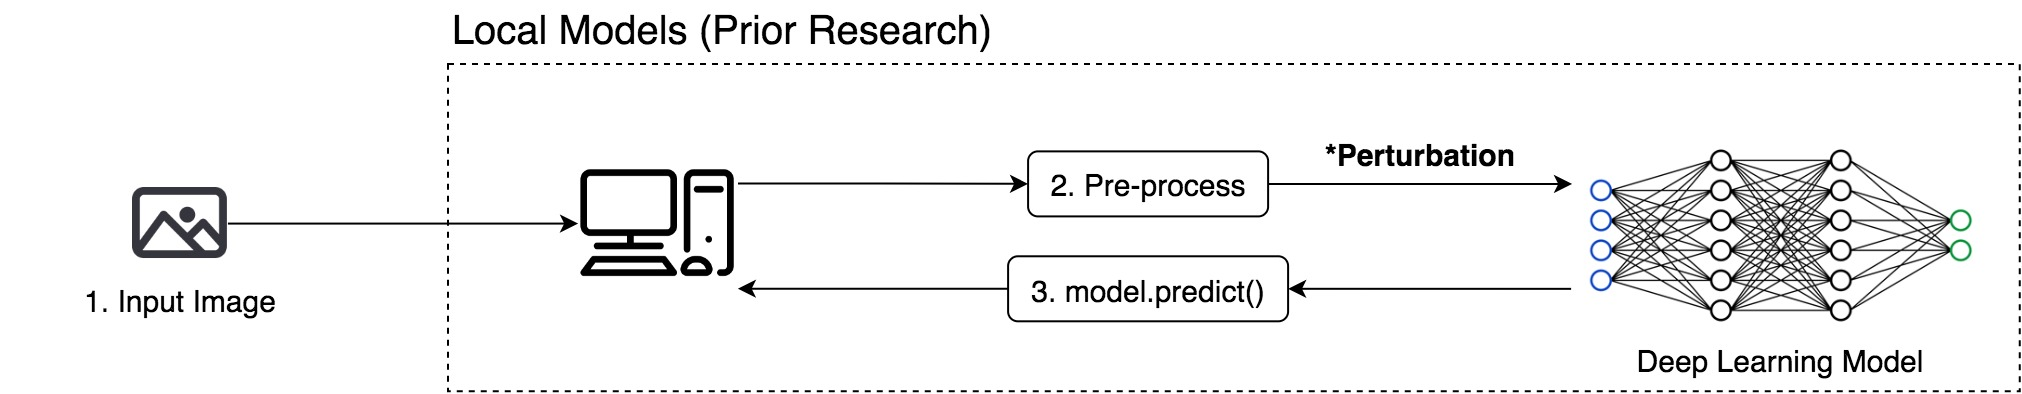
\includegraphics[width=\linewidth]{figures/chapter_classification/local.jpg}
    \caption{\textbf{Attacking Local Models}: Most prior research attacked local models and applied the adversarial perturbation after image resizing and pre-processing, assuming access to input shapes of black-box models.}
    \label{fig:local}
\end{figure}

\begin{figure}[H]
    \centering
    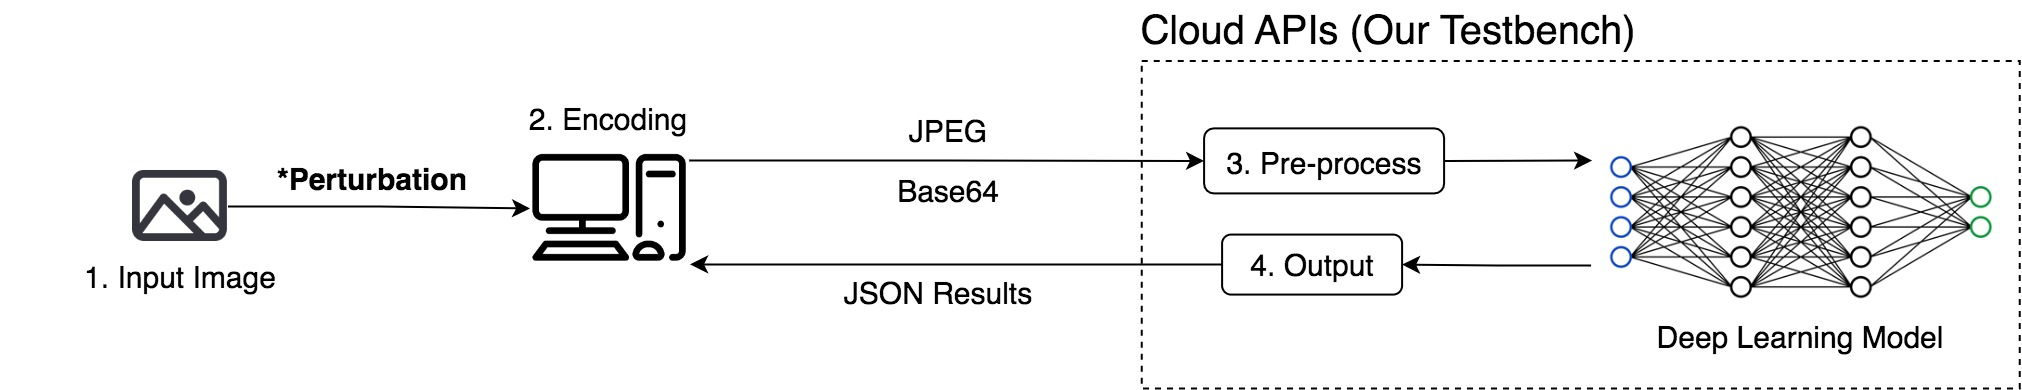
\includegraphics[width=\linewidth]{figures/chapter_classification/cloudapi.jpg}
    \caption{\textbf{Attacking Cloud APIs}: We initiate black-box attacks directly against cloud services and apply the perturbation before image encoding and pre-processing, assuming no access to the internal design of commercial APIs.}
    \label{fig:cloudapi}
\end{figure}

% \begin{figure}[H]
%     \begin{subfigure}[bp]{\textwidth}
%         \centering
%         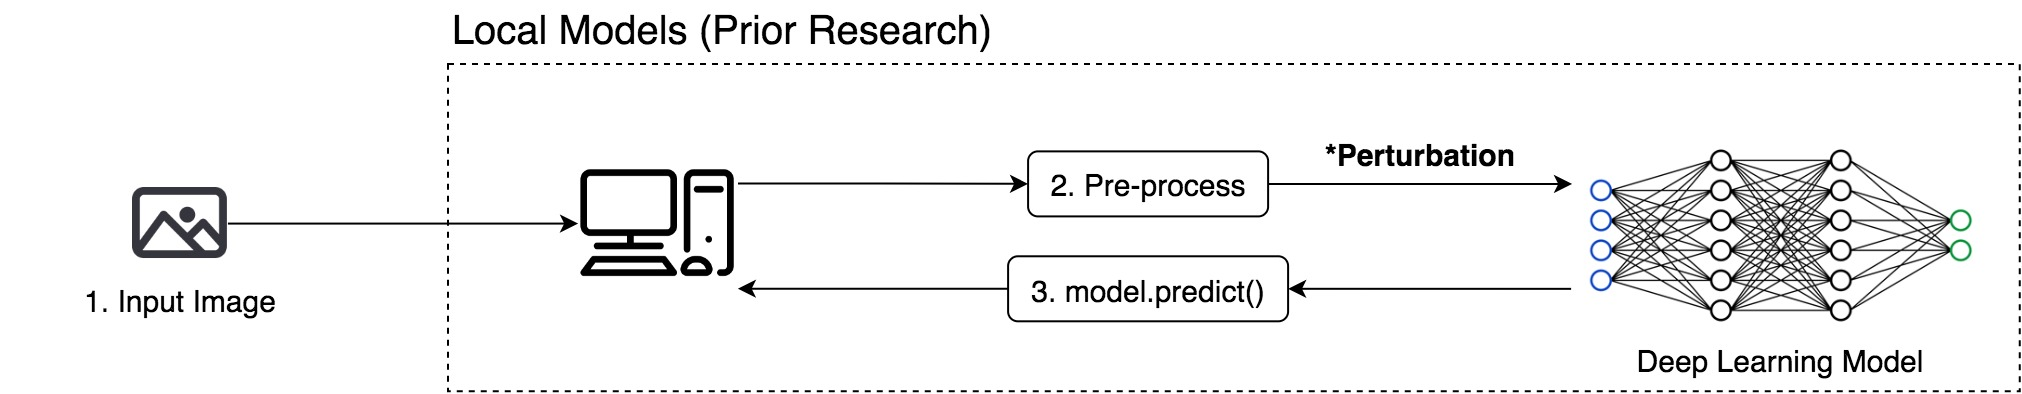
\includegraphics[width=\linewidth]{figures/chapter_classification/local.jpg}
%         \caption{Most prior research attacked local models and applied the perturbation after image resizing and pre-processing, assuming access to input shapes of black-box models.}
%         \label{fig:local}        
%     \end{subfigure}
%     \begin{subfigure}[bp]{\textwidth}
%         \centering
%         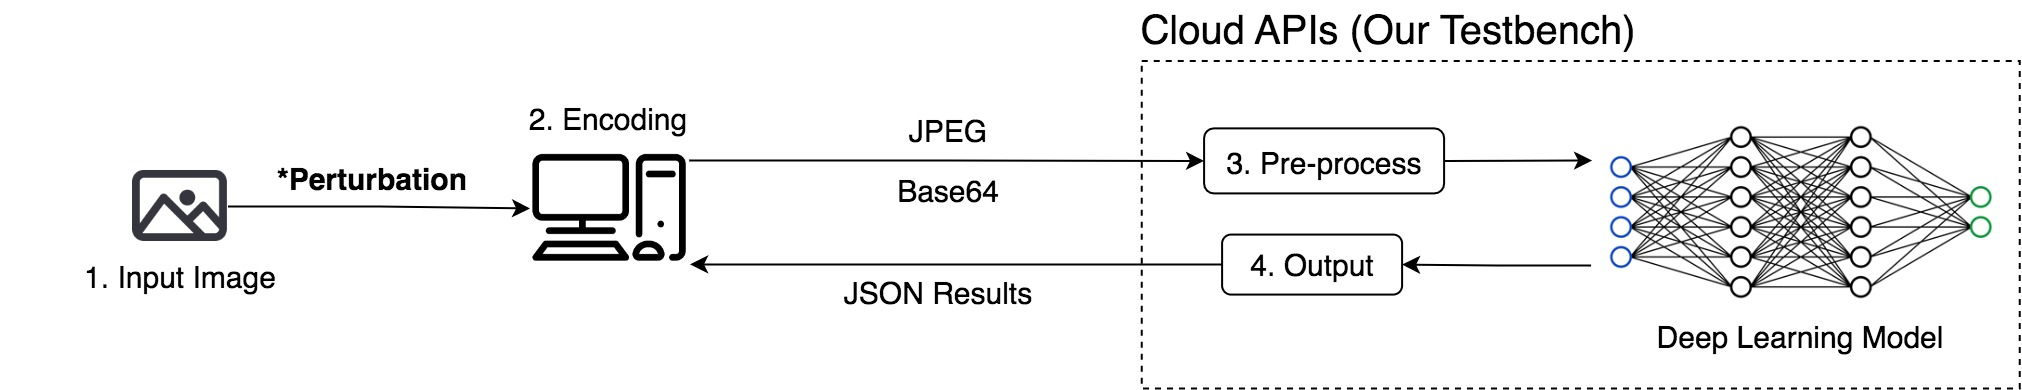
\includegraphics[width=\linewidth]{figures/chapter_classification/cloudapi.jpg}
%         \caption{We initiate the black-box attacks directly against cloud services and apply the perturbation before image encoding and pre-processing.}
%         \label{fig:cloudapi}
%     \end{subfigure}
%     \caption{The difference}
% \end{figure}

\clearpage

\subsection{Common Mistakes}
\label{common_errors}

During our implementation of distributed black-box attacks, we observed that some previous research made certain errors in the query process, which provided their attacks with an unfair advantage. This advantage led these methods to outperform state-of-the-art black-box attacks, but it was based on the assumption of accessing information that is not available for black-box attacks. 

For instance, the Bandits Attack \citep{ilyas2018black, ilyas2018prior} applied image resizing and center cropping before initiating the attack, indicating adversaries have access to the input shape and pre-processing methods of a black-box model. The HopSkipJump Attack \citep{chen2020hopskipjumpattack}, on the other hand, tested their attacks on images that share the same input shape, such as MNIST (28x28x1), cifar10 and cifar100 (32x32x3). Although the Biased Boundary Attack \citep{Brunner_2019} was tested on ImageNet, which includes images of different input shapes, the attack resized all images to the input shape for Inceptionv3 (299x299x3). Our experimental results reveal a significantly lower attack success rate if the attack is initiated on the original input image before the image pre-processing.

We found similar mistakes in other research on black-box attacks, such as Square Attack \citep{andriushchenko2020square}, Parsimonious Attack \citep{moon2019parsimonious}, SimBA Attack \citep{guo2019simple}, Geometric Decision-based Attack \citep{rahmati2020geoda}, etc \citep{cheng2018query, cheng2019sign, chen2020rays, debenedetti2023evading}. Some papers did not provide the source code, but example images in the paper share the same shape \citep{chen2023query, bai2023query, xu2023sparse, wu2023black}, indicating the possible existence of similar mistakes. These mistakes could also exist in black-box attacks against other deep learning applications, such as video recognition \citep{jiang2019black, chen2023coreset, mu2024enhancing}, face recognition \citep{dong2019efficient, ma2023transferable}, NLP neural ranking \citep{wu2023prada, liu2022order} and 3D point cloud \citep{liu2022imperceptible, zhang20233d, tao20233dhacker}.

Most prior research tests their attacks on local models rather than Cloud APIs because it is faster and less costly (large-scale querying against commercial APIs is non-free). Thus, they tested their attacks on local models and relied on themselves to restrain access to extra model information. These attacks achieve significantly lower success rates when attacking cloud services due to the following reasons.

\textbf{Image Encoding}: In real-world scenarios, images are typically encoded before being sent to cloud services to reduce the amount of data transmitted and to save bandwidth (see Fig. \ref{fig:cloudapi}). However, prior research often assumes that perturbations can be added directly to the raw input image (see Fig. \ref{fig:local}). 

It is worth noting that cloud services such as Google Cloud Vision and Imagga accept raw binary and base64 encoded JPEG (lossy compression) images as input. This compression may cause part of the adversarial perturbations to be ineffective, ultimately reducing the success rate of attacks. Therefore, if we evaluate black-box attacks on local models without considering image encoding and quantization, we may overestimate the effectiveness of these attacks. % against real-world cloud APIs.

Besides, image classification cloud services do not accept images with invalid pixel values. For example, the Bandit Attack does not clip the image while estimating gradients, assuming they can send invalid images (pixel value $>$ 255 or $<$ 0) to the black-box model.

\textbf{Image Pre-processing}: Some papers apply perturbations \emph{after} image resizing, thereby assuming that they know the input shape of the image classification model in the cloud. Moreover, note that original input images are typically larger than the model input size. Resizing high-resolution images to a lower resolution reduces the sampling space. Therefore, it is less computationally intensive to generate perturbations after image resizing.

\subsection{Possible Causes}

Sending queries to real-world cloud APIs typically costs around \$1 for every 1,000 requests (for example, using Google Cloud Vision). In other words, an experiment attacking 1,000 images may require 1,000,000 queries and cost \$1,000. Thus, most prior research tested their attacks on local models. However, intentionally or unintentionally, they exploit extra information that improves their attacks due to the following reasons:

\begin{itemize}
    \item The model prediction function accepts raw images as float numbers and will not give an error even if the input image $x$ contains negative values. Thus, prior research did not encode input images and was unaware that invalid images were sent to the model.
    \item The model prediction function only accepts input images $x$ as an array of the same shape. It is tempting to resize all input images to the same size as the model input, thus unintentionally exploiting extra information about the model input shape.
\end{itemize}

As a result, some prior research tested their attacks on local models and compared their methods with others with unfair settings. 

% In the next section, we introduce our open-source image classification cloud service. This cloud service will both facilitate future research and prevent these mistakes so that we can obtain a fair comparison of existing black-box attacks.

\clearpage

\subsection{Contributions}

This paper aims to investigate if black-box adversarial attacks have become a practical threat against image classification cloud services. Our main contributions are as follows: 

\begin{itemize}
    \item We identify some common mistakes in prior research that leads to an overestimation of the efficiency of black-box attacks. To avoid these mistakes, we design an image classification cloud API for benchmark, and we open source this cloud API for future research on black-box attacks
    \footnote{The source code of DeepAPI is available on Github: \url{https://github.com/wuhanstudio/deepapi}.}.
    % \footnote{The source code of DeepAPI is available on Anonymous GitHub: \url{https://anonymous.4open.science/r/DeepAPI-6832}.}.
    \item We design a framework that facilitates horizontally and vertically distributed queries to speed up online attacks against cloud APIs (see Fig. \ref{fig:distributability})
    \footnote{The source code of the online black-box attacks is available on Github: \url{https://github.com/wuhanstudio/adversarial-classification}.}. 
    % \footnote{The source code of the online black-box attacks is available on Anonymous GitHub: \url{https://anonymous.4open.science/r/adversarial-classification-F32B}.}. 
    \item We also provide an open-source Black-box Adversarial Toolbox that simplifies the process of conducting black-box attacks against cloud APIs
    \footnote{The source code of the black-box adversarial toolbox is available on Github: \url{https://github.com/wuhanstudio/blackbox-adversarial-toolbox}.}.
    % \footnote{The source code of the black-box adversarial toolbox is available on Anonymous GitHub: \url{https://anonymous.4open.science/r/blackbox-adversarial-toolbox-6A8C}.}. 
    
\end{itemize}

\begin{figure}[H]
    \centering
    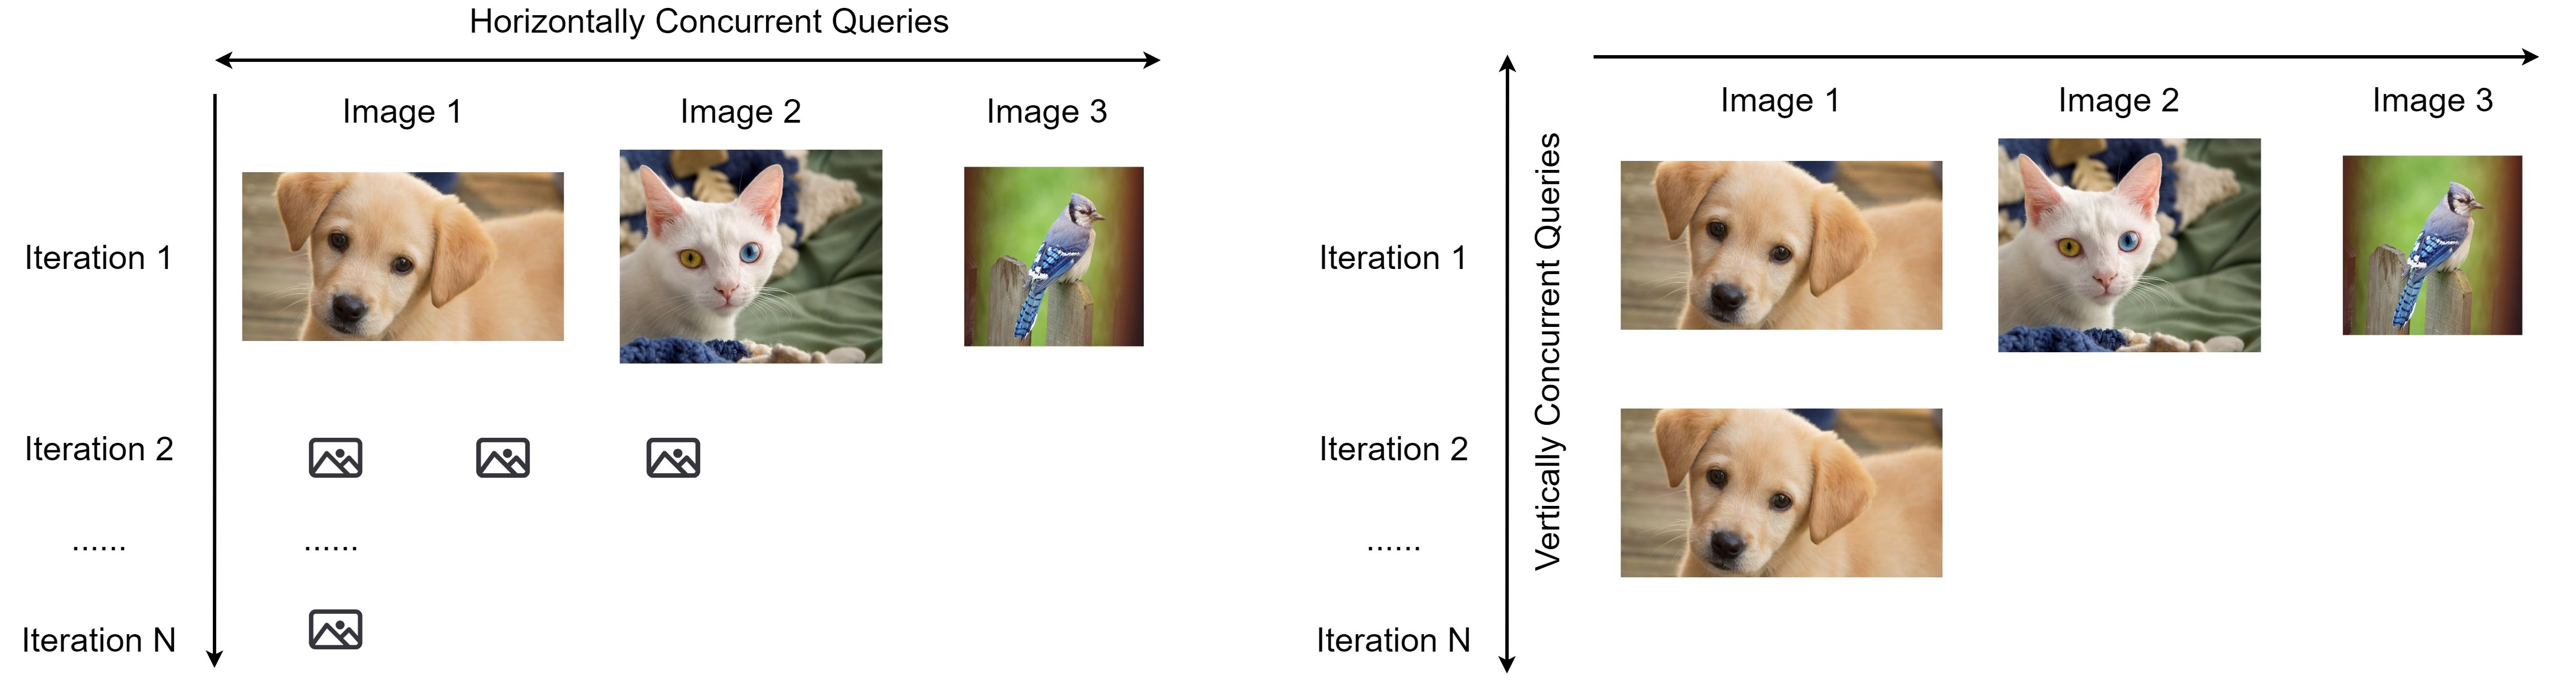
\includegraphics[width=\linewidth]{figures/chapter_classification/distribution.jpg}
    \caption{The difference between horizontal and vertical distribution.}
    \label{fig:distributability}
\end{figure}


\section{Preliminaries}

\subsection{Image Classification Models}

The state-of-the-art image classification models that use convolutional neural networks (CNN) achieve a Top-1 accuracy of over 90\% and a top-5 accuracy of over 99\% on the ImageNet dataset \citep{pham2021meta}. Among them, ResNet \citep{he2016deep}, MobileNet \citep{howard2017mobilenets}, InceptionV3 \citep{szegedy2016rethinking}, and EfficientNet \citep{tan2019efficientnet} are the most popular models for real-world applications, as they balance model size and accuracy well. 

Previous research on black-box adversarial attacks against image classification models has mainly focused on VGG16 \citep{simonyan2014very}, ResNet50, and InceptionV3, pre-trained on the ImageNet \citep{russakovsky2015imagenet} dataset.

\textbf{VGG16}: The VGGNet is well known for its simplicity. 3x3 convolutional layers and a max-pooling layer are stacked on each other as a sequential model, followed by three fully-connected layers. Being 16 layers deep, VGG16 was considered to be a very deep neural network when it was introduced in 2014. Today, however, improvements in computational resources enable even deeper neural networks to be implemented.

\textbf{ResNet50}: In 2015, ResNet made it possible to train up to hundreds or even thousands of layers. The residual building block introduces skip connections to solve the vanishing gradient problem in deep CNNs, while preserving the overall performance. In research on black-box adversarial attacks, ResNet50 is one of the most widely used variants.

\textbf{Inceptionv3}: Choosing the kernel size for convolution layers is tricky. The use of different kernel sizes in different layers may both exacerbate the vanishing gradient problem and lead to higher requirements on the computational resources. The inception module instead puts several convolution layers with different kernel sizes side-by-side at the same level and introduces extra 1x1 convolutions to control the number of features. Besides, an auxiliary loss is added to the original loss to avoid the vanishing gradient problem. The inception module was introduced by Google, and thus, the first version is known as GoogleNet.

% Section \ref{section_experimental_evaluation} describes experiments for evaluating the efficiency of horizontally and vertically distributed attacks against image classification cloud services utilizing VGG16, ResNet50, or InceptionV3.

All the three models described above are vulnerable to black-box adversarial attacks \citep{szegedy2013intriguing, biggio2013evasion}. This paper introduces distributed black-box attacks to investigate if black-box attacks could be real threats against image classification cloud services.


\subsection{Black-box Adversarial Attacks}
\label{black_box}

Black-box attacks aim to deceive deep-learning models without having access to their internal structure or weights. Two common types of black-box attacks are gradient estimation and local search methods, which have been widely studied in the literature \citep{bhambri2019survey} \citep{wang2022black}.

% \textbf{Problem Formulation}: Given some input image $x$ and true labels $y$, the objective of the adversary is to add a small perturbation $\delta$ to the original image, and generate an adversarial image $x' = x\ +\ \delta$ that can fool a black-box image classifier $C(x)$, such that $C(x') \neq C(x)$. Typically, the perturbation $\delta$ is bounded in the $l_2$ or $l_\infty$ norm by some user-defined constant \citep{bhambri2019survey}. In addition, the adversary does not know the model structure and weights. 

% Further, the attacker has limited access to model outputs for black-box models deployed on cloud servers. For example, in the partial-information setting, the adversary only has access to the prediction probabilities of the top $k$ classes $\{y_1, ..., y_k\}$. In the label-only setting, the adversary can only access the prediction label without any knowledge of prediction probabilities \citep{ilyas2018black}.

\textbf{Local Search Methods}: The task of generating adversarial inputs can be approached as a problem of selecting what pixels to attack. Thus, we can use existing local search methods to search for combinations of pixels to be perturbed. One simple, yet effective, baseline attack that use this idea is the simple black-box attack (SimBA) \citep{guo2019simple}. With SimBA, a vector is randomly sampled from a predefined orthonormal basis and then added or subtracted from the image. To improve sample efficiency, Andriushchenko et al. proposed the square attack \citep{andriushchenko2020square}. This attack initializes the perturbation using vertical stripes, since CNNs are sensitive to high-frequency perturbations \citep{yin2019fourier}, and then generates square-shaped perturbations at random locations to deviate model classifications.

\textbf{Gradient Estimation Methods}: Inspired by white-box attacks that use gradients to generate adversarial perturbations \citep{GoodfellowSS14} \citep{madry2017towards}, black-box gradient estimation methods estimate gradients through queries, and then use these estimated to construct adversarial perturbations. To estimate gradients, Chen et al. used the finite-differences method to compute the directional derivative at a local point \citep{chen2017zoo}. To improve query efficiency, Ilyas et al. proposed a natural evolutionary strategy (NES) \citep{wierstra2014nes} based method to approximate gradients, and proved that the standard least-squares estimator is an optimal solution to the gradient-estimation problem \citep{ilyas2018black}. In the Bandits attack, Ilyas et al. further improved the classifier by using priors on the gradient distribution \citep{ilyas2018prior}, thereby exploiting the fact that the gradients at the current and previous steps are highly correlated.

% \begin{figure}[b]
%     \centering
%     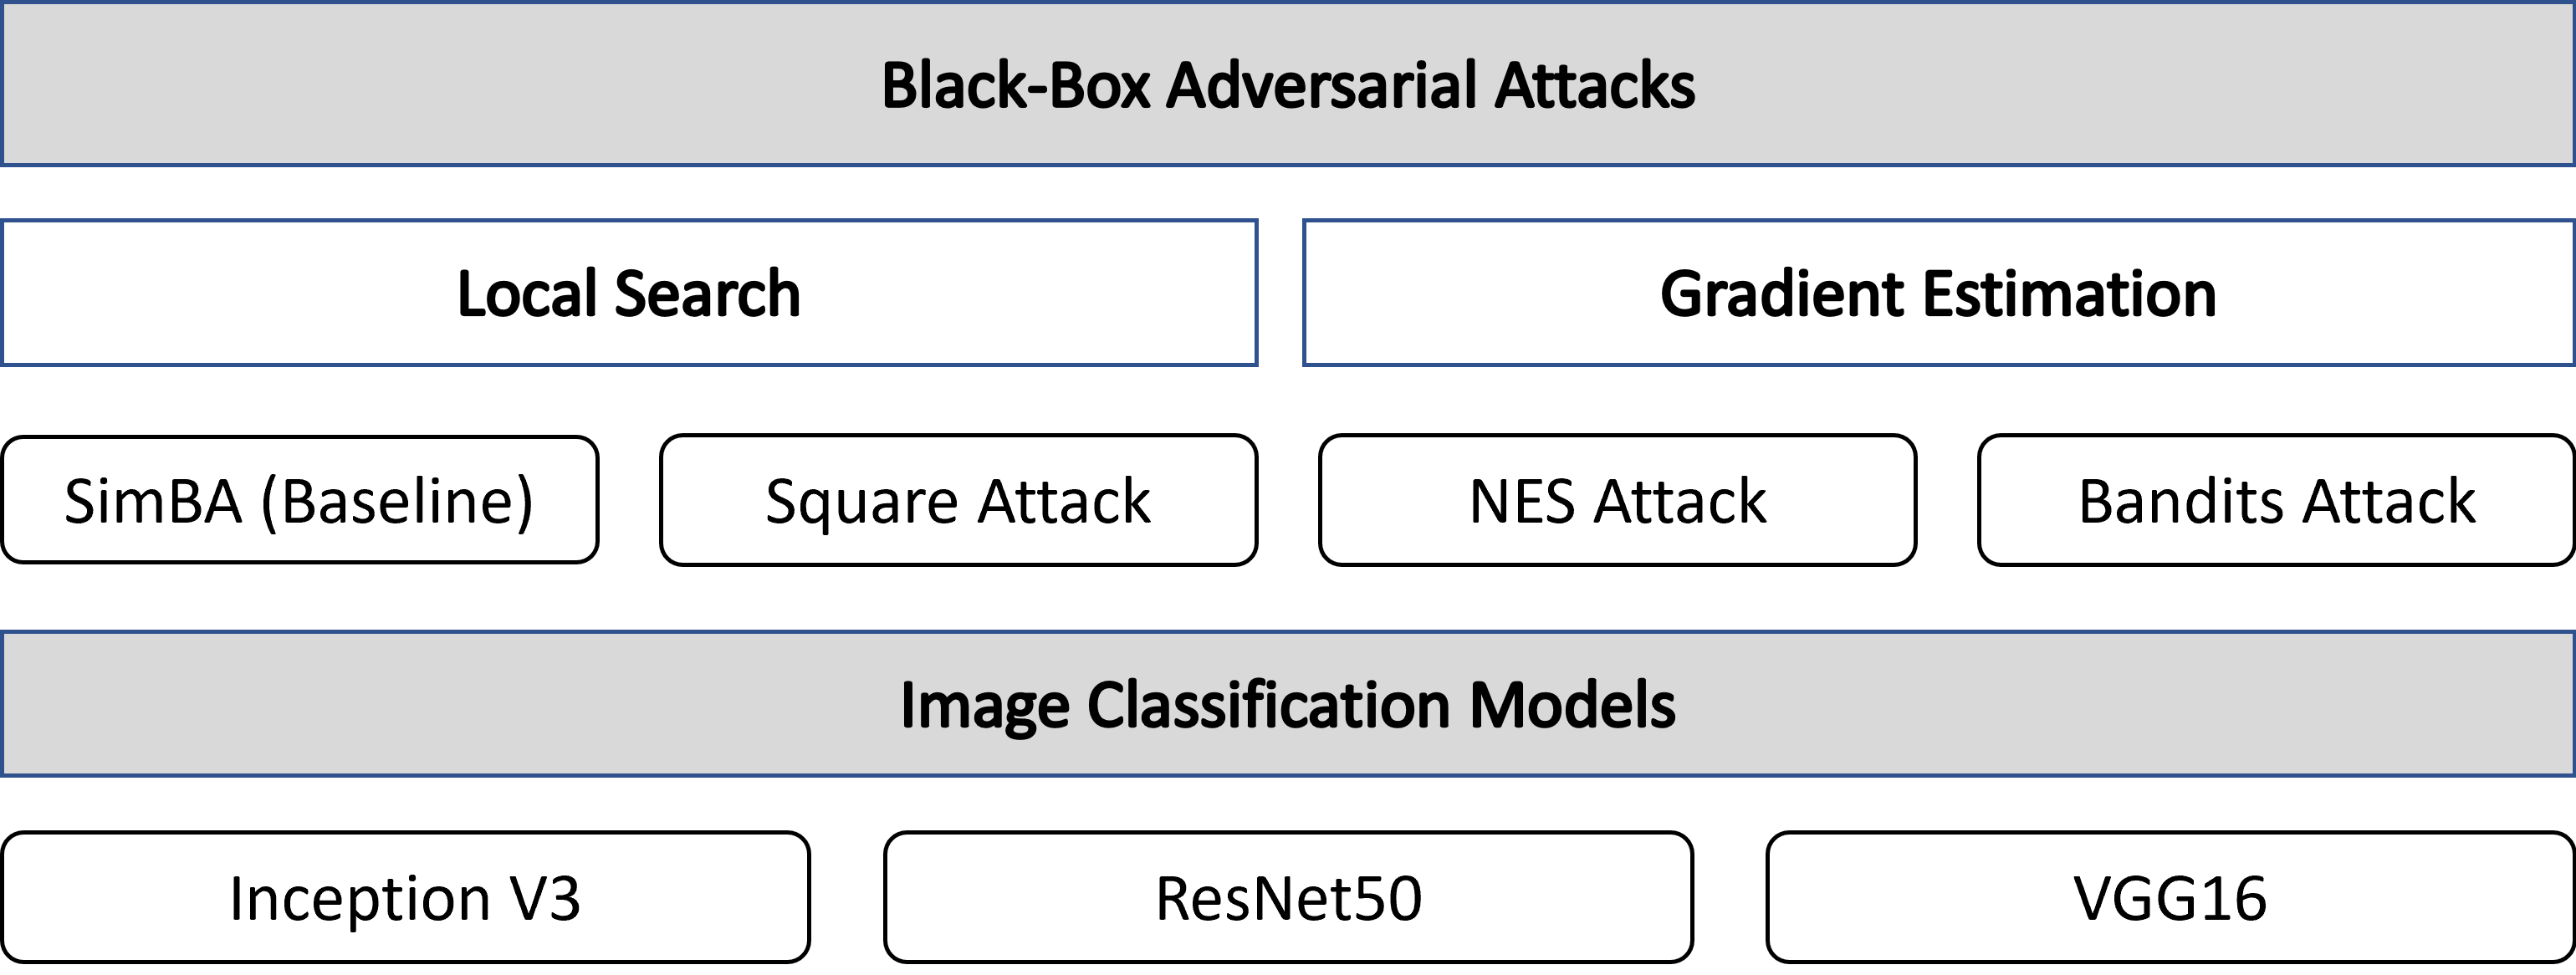
\includegraphics[width=0.5\textwidth]{figures/chapter_classification/overview.png}
%     \caption{An overview of black-box attacks and classification models tested in this paper.}
%     \label{fig:overview}
% \end{figure}

% \clearpage

\section{Distributed Black-box Attacks}

\subsection{Problem Formulation}

Given some input image $x$ and true labels $y$, the objective of the adversary is to add a small perturbation $\delta$ to the original image, and generate an adversarial image $x' = x\ +\ \delta$ that can fool a black-box image classifier $C(x)$, such that $C(x') \neq C(x)$. Typically, the perturbation $\delta$ is bounded in the $l_2$ or $l_\infty$ norm by some user-defined constant \citep{bhambri2019survey}.

The adversary does not know the model structure and weights. Further, the attacker has limited access to model outputs for black-box models deployed on cloud servers. For example, in the partial-information setting, the adversary only has access to the prediction probabilities of the top $k$ classes $\{y_1, ..., y_k\}$. In the label-only setting, the adversary can only access the prediction label without any knowledge of prediction probabilities \citep{ilyas2018black}.

\subsection{Distributed Queries}

Cloud computing platforms serve APIs via load balancing: several computing engines simultaneously provide the same model-inference service. If we exploit load balancing and send multiple queries concurrently, we can receive all the results simultaneously and thus accelerate black-box attacks significantly.

To demonstrated this hypothesis, we sent 1, 2, 10, and 20 queries concurrently to Google Cloud Vision, Imagga, and DeepAPI (see Fig. \ref{fig:dist_query}). Since the PC has eight cores, we sent concurrent queries from eight workers. Tab. \ref{table_query} lists the total time, averaged over 10 experiments, before receiving all responses. As can be seen, the total time does not grow linearly with the number of queries. Rather, the average query time decreases as we send out more concurrent queries.

Black-box attacks are usually slow because they require several thousands of queries. Depending on the network quality, it could take 0.5$-$2s to receive one query result from an API server, and thus, it could take several hours to launch a black-box attack. However, cloud computing platforms serve APIs via load balancing, which means that several computing engines provide the same model-inference service simultaneously. If we exploit load balancing and send multiple queries concurrently, we can receive all the results simultaneously and thus accelerate black-box attacks significantly. 

In conclusion, thanks to load balancing, the more queries we send, the faster the queries become on average. This is a feature that we will exploit to accelerate black-box attacks. 


\begin{figure}[H]
    \centering
    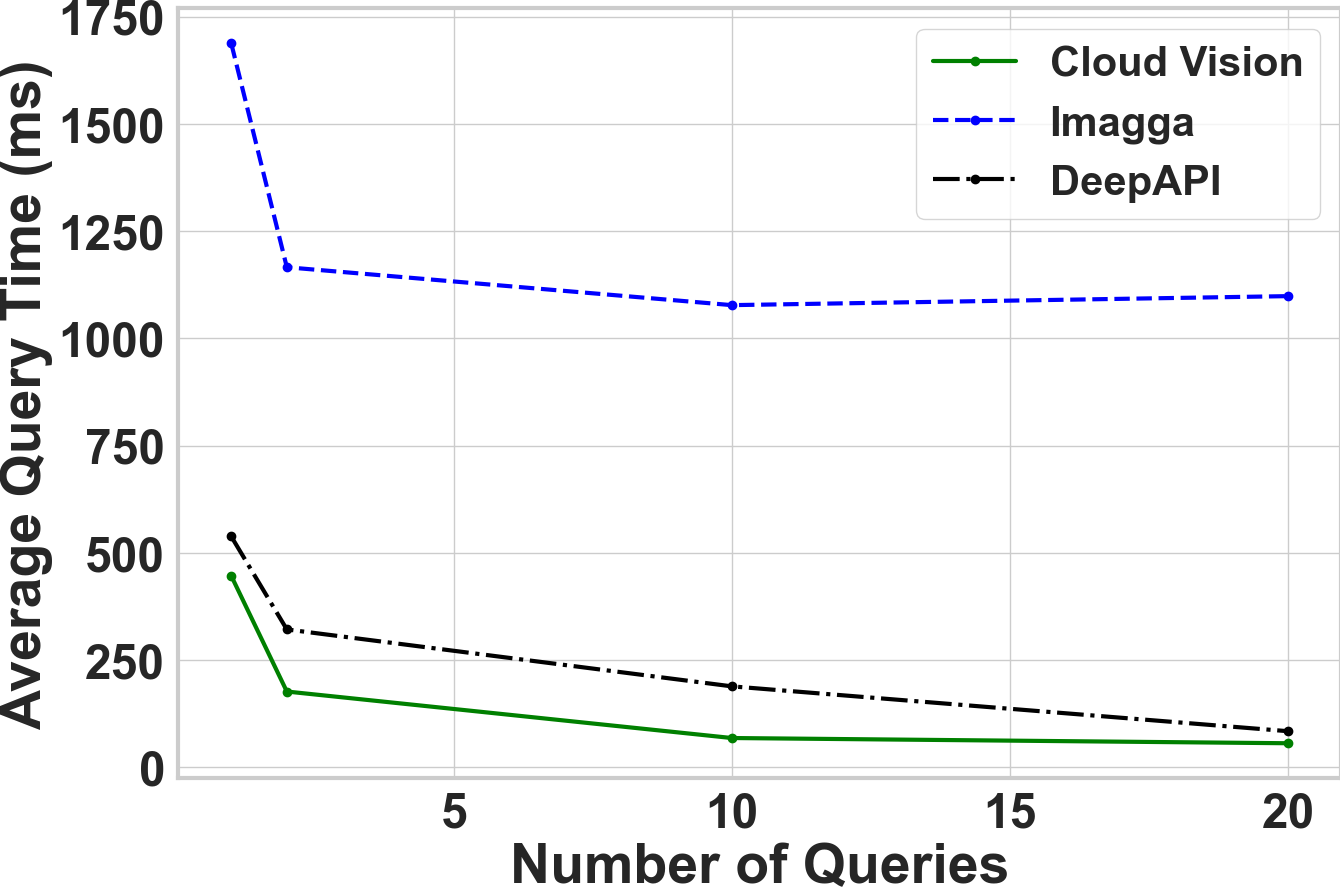
\includegraphics[width=0.8\textwidth]{figures/chapter_classification/average_query_time.png}
    \caption{The average query time when sending concurrent queries to cloud APIs.}
    \label{fig:dist_query}
\end{figure}

\begin{table}[H]
\begin{center}
\begin{tabular}{cca}
    \hline
    Queries       & \multicolumn{2}{c}{Google Cloud Vision} \\
    \hline
    & Total Time & Average Time \\
    \hline
    1      & 446.7ms   & 446.7ms \\
    2      & 353.61ms  & 176.8ms \\
    10     & 684.25 ms & 68.4ms  \\
    20     & 1124.82ms & 56.2ms  \\
    \hline
    % 
    \multicolumn{3}{c}{\vspace{0.5cm}} \\
    % 
    \hline
    Queries     & \multicolumn{2}{c}{Imagga} \\
    \hline
    & Total Time & Average Time \\
    \hline
    1      & 1688.1ms  & 1688.1ms \\
    2      & 2331.81ms & 1165.9ms \\
    10     & 10775.8ms & 1077.6ms \\
    20     & 21971.8ms & 1098.6ms \\
    \hline
    % 
    \multicolumn{3}{c}{\vspace{0.5cm}} \\
    % 
    \hline
    Queries      & \multicolumn{2}{c}{DeepAPI (Ours)} \\
    \hline
    & Total Time & Average Time \\
    \hline
    1      & 538.5ms  & 538.5ms \\
    2      & 643.2ms  & 321.6ms \\
    10     & 1777.8ms & 177.8ms \\
    20     & 1686.4ms & 84.3ms  \\
    \hline
\end{tabular}
\end{center}
\caption{The total and average time of sending concurrent queries to cloud APIs.}
\label{table_query}
\end{table}

% \pagebreak

% \subsection{DeepAPI}

% To facilitate future research on distributed black-box attacks that attack cloud APIs rather than local models, we designed DeepAPI, an open-source image classification cloud service (see Fig. \ref{fig:deepapi}) that supports:

% \begin{itemize}
%     \item The three most popular classification models (VGG16, ResNet50, and Inceptionv3) for research on black-box attacks provided by Keras Model Zoo \citep{chollet2015keras}.
%     \item Both soft labels (with probabilities) and hard labels (without probabilities).
%     \item Top $k$ predictions ($k \in \{1, 3, 5, 10\}$) for partial-information setting.
%     % \item A Web UI as well as distributed API requests.
% \end{itemize}

% \begin{figure}[btp]
%     \centering
%     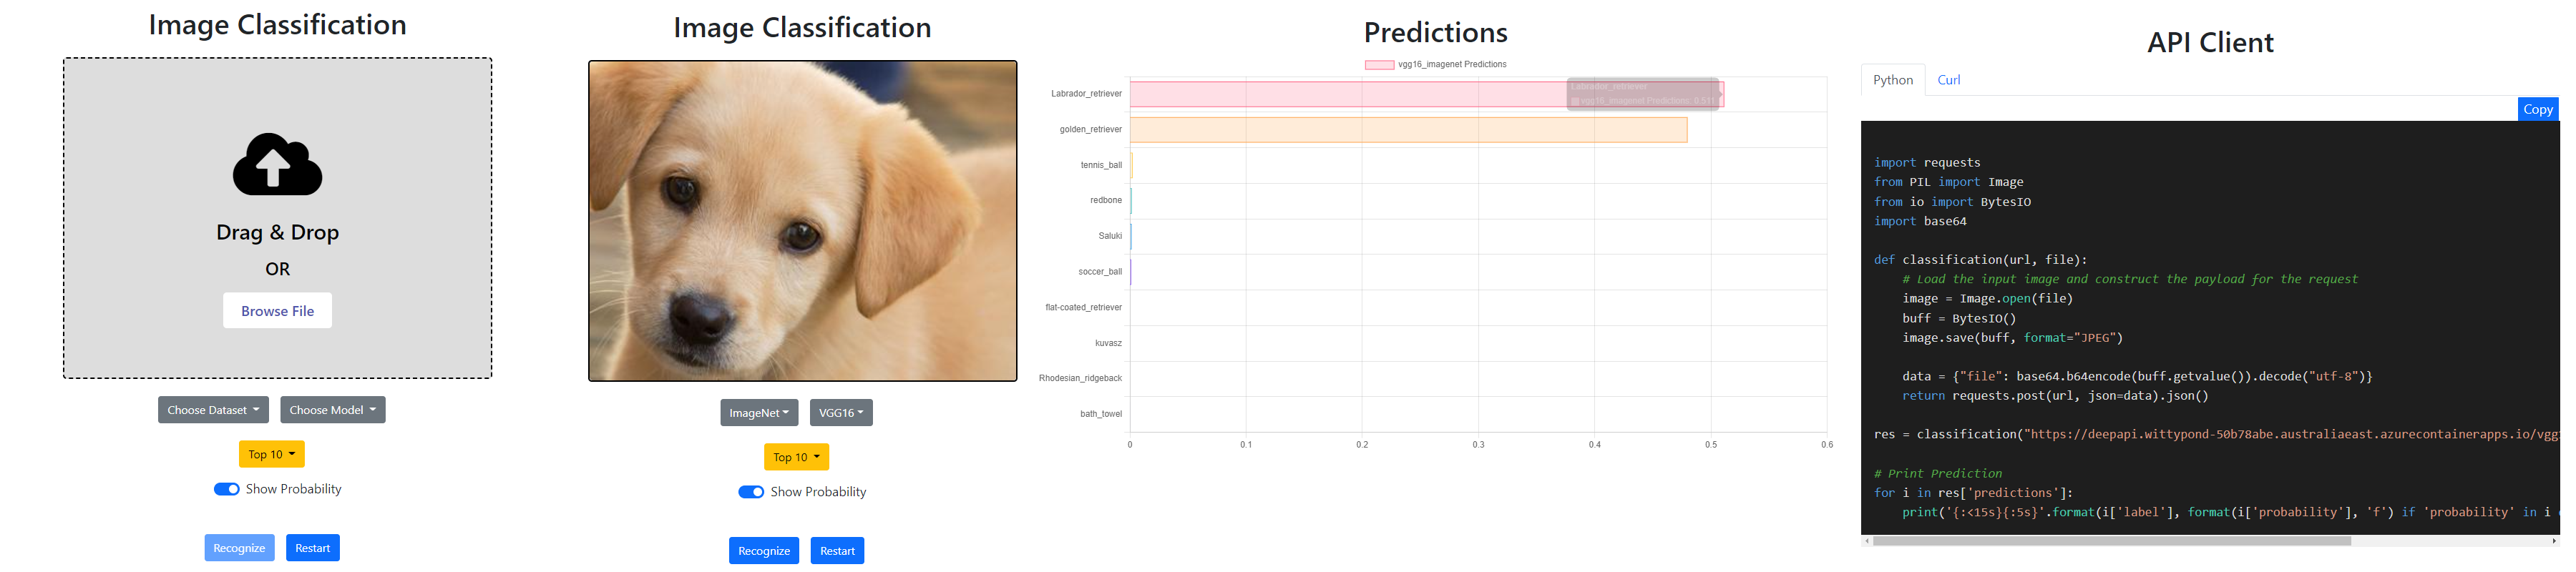
\includegraphics[width=\linewidth]{figures/chapter_classification/deepapi.png}
%     \caption{DeepAPI provides both web interface and APIs for research on black-box attacks.}
%     \label{fig:deepapi}
% \end{figure}

\subsection{Horizontal and Vertical Distribution}
\label{horizon_vertical}

Both local (multi-core CPU) and cloud-based (load balancer) deep learning models are vulnerable to distributed queries, but the challenge lies in deciding which queries to send concurrently. To address this problem, we propose horizontal and vertical distribution for black-box attacks, inspired by horizontal and vertical scaling of cloud resources \citep{Millnert2020}.

Horizontal distribution concurrently sends queries for different images within the same iteration, thereby allowing the generation of multiple adversarial examples concurrently. This can be achieved without altering existing black-box attack methods. We can apply horizontal distribution by implementing a distributed query function that sends concurrent requests to cloud APIs. 

Vertical distribution, on the other hand, sends multiple concurrent queries for the same image, thereby accelerating the attack for that particular image. Existing black-box attack methods need to be redesigned to decouple the queries across iterations. We use SimBA, Bandits Attack and Square Attack as exmaples to illustrate how to apply vertical distributions to existing black-box attacks.

In summary, horizontal distribution achieves concurrent attacks against multiple images, while vertical distribution speeds up attacks on a single image (see Fig. \ref{fig:distributability}). Since horizontal distribution does not require significant modifications to the original attack method, we focus on vertical distribution in the following sections. 

\begin{figure}[H]
\begin{minipage}{\textwidth}
\begin{algorithm}[H]
    \centering
    \caption{Horizontal Distribution}
    \label{alg:horizontal}
    \begin{algorithmic}[1]
        \State {\bf Input}: Input images $x \in X$, and the maximum number of iterations $n_{iter}$ for each image.
        \State {\bf Output}: Adversarial images $x' \in X'$. 
        \State
        \State Initialize: $X^{'}$.
        \For {each iteration $n \in [0,\ n_{iter})$}
        \State //\ Concurrent requests across images.
            \State $X^{'}$ = Black\_Box\_Attack$(X$, y)
            \State \{
            % \bindent
                \State \hspace{\algorithmicindent}Update $X^{'}$.
                \State \hspace{\algorithmicindent}Concurrent Queries: y{'} = C($X{'}$).
            % \eindent
            \State \}
            \State \textbf{if} {success rate == 100\%} \textbf{then} {\textbf{break}}.
        \EndFor
    \end{algorithmic}
\end{algorithm}
\end{minipage}
\end{figure}

\subsection{Distributed SimBA (Baseline Method)}

We first use a baseline method, SimBA \citep{guo2019simple}, to illustrate how to apply vertical distribution. In each iteration, SimBA increases or decreases the value of one randomly chosen pixel, and assumes that for any perturbation vector $\boldsymbol{q}$ and some step size $\epsilon$, either $x + \epsilon\boldsymbol{q}$ or $x - \epsilon\boldsymbol{q}$ will decrease the highest probability $p_h(x')$ in $y = C(x')= (p_1, p_2, ..., p_K)$. Thus, we can randomly pick a vector $\boldsymbol{q}$ in the set of orthogonal search directions $Q$ and then either add or subtract it from the image $x$ to decrease the highest probability $p_h(x')$. To guarantee maximum query efficiency, $\boldsymbol{q}$ are picked from $Q$ without replacement, and all vectors in $Q$ are orthonormal.

% Horizontal distribution does not require any significant modifications to the original attack method. We apply horizontal distribution by implementing a distributed query function that sends concurrent requests to cloud APIs.

To apply vertical distribution to SimBA, we need to decouple the correlation between queries at different iterations. The original SimBA generates perturbations pixel by pixel. After receiving previous query results and deciding the perturbation $\delta \in \{-\boldsymbol{q}\epsilon, +\boldsymbol{q}\epsilon\}$ for each vector $\boldsymbol{q}$, the algorithm then goes on to choose which pixel to perturb in the next iteration. To decouple the correlation, we devise vertically distributed SimBA that sends out queries for several perturbation vectors $\boldsymbol{q}$ as a batch $\boldsymbol{q}_{batch}$ concurrently. The sign of each perturbation vector is decided independently. Then, we sum and project the accumulated perturbation $\delta$ to the $L_2$ ball at the end of each iteration to guarantee imperceptibility (see Alg. \ref{alg:simba_vertical}). 

% \clearpage

\begin{figure}[H]
\begin{minipage}{\textwidth}
\begin{algorithm}[H]
    \centering
    \caption{Distributed SimBA (Vertical)}
    \label{alg:simba_vertical}
    \begin{algorithmic}[1]
        \For {each image $x_{i} \in X$}
            \State $x'_{i},\ y'_{i}$ = SimBA($x_{i}$, $y_{i}, Q, \alpha, \epsilon, n_{batch}$)
            % \State \{
            \Indent
                \State Initialize: $\delta_i = 0, x'_{i} = x_i + \delta_i$.
                \For {each iteration $n \in [0,\ n_{iter})$}
                    \State \text{Pick $\boldsymbol{q}_{batch} \in Q$ randomly without replacement.}
                    % \State
                    \State //\ Concurrent requests across iterations.
                    \State $p^+ = C(x{'} + \boldsymbol{q}_{batch}\epsilon$).
                    \State $p^- = C(x{'} - \boldsymbol{q}_{batch}\epsilon$).
                    % \State
                    \For{$\boldsymbol{q}_i \in \boldsymbol{q}_{batch}$}
                        \If {$p_{i}^+ < \boldsymbol{y}'_i$}
                            \State \text{$\delta^{'}_i = \delta^{'}_i + \alpha \boldsymbol{q}_i$} 
                        \ELSIF{$p_{i}^- < \boldsymbol{y}'_i$}
                            \State \text{$\delta^{'}_i = \delta^{'}_i - \alpha \boldsymbol{q}_i$} 
                        \EndIf
                    \EndFor
                    % \State
                    \State $\delta_i = proj_{p}(\delta_i)$
                    \State $x'_i = x'_i + \delta_i$
                    % \State Update $y_i^{'}$.
                    \State $n = n + n_{batch}$
                    \State \textbf{if} {success} \textbf{then} {\textbf{break}}.
                \EndFor
            \EndIndent
            % \State \}
        \EndFor
    \end{algorithmic}
\end{algorithm}
\end{minipage}
\end{figure}

% \clearpage

\subsection{Distributed Square Attack (Local Search)}

The square attack is a local search method that is more query-efficient than SimBA and achieves SOTA attack success rate \citep{andriushchenko2020square}. 

The square attack improves query efficiency by initializing the perturbation with vertical stripes, motivated by the fact that CNNs are sensitive to high-frequency perturbations \citep{yin2019fourier}. Then, the square attack generates square-shaped perturbations to decrease the margin loss $L(C(X), y)$ defined by:
\begin{equation}
L(C(X), y) = C_y(X) - \max_{k \neq y}C_k(X)    
\end{equation}
where $y$ is the correct class of the input image X and $C_k(X)$ is the output probability of class $k$.

We apply horizontal distribution to both the initialization and iteration processes across images. To apply vertical distribution, we generate a batch of square-shaped perturbations independently and send out queries concurrently for each perturbation. After receiving the queries, we add the perturbations that reduce the margin loss $L(C(X^{'}), y)$ to the image. Then, we project the accumulated perturbation to the $L_\infty$ ball to ensure imperceptibility (see Alg. \ref{alg:square_vertical}).

% The vertically distributed square attack decouples the dependency across iterations by generating a batch of square-shaped perturbations independently and then only applying perturbations that decrease the margin loss. To ensure imperceptibility, we project the perturbation to the $L_\infty$ ball after applying each square-shaped perturbation (see Algorithm \ref{alg:square_vertical}).

\begin{figure}[H]
\begin{minipage}{\textwidth}
\begin{algorithm}[H]
    \centering
    \caption{Distributed Square Attack (Vertical)}
    \label{alg:square_vertical}
    \begin{algorithmic}[1]
        \For {each image $x_{i} \in X$}
            \State Initialize: $x'_{i} = init(x_{i})$ with vertical strips.
            \State Single Query: $l^{*}_i = L(C(x'_i), y)$.
            \State $x'_{i},\ y'_{i}$ = SquareAttack($x_{i}$, $y_{i},\epsilon, n_{batch}$):
            % \State \{
            \Indent
                \For {each iteration $n \in [0,\ n_{iter})$}
                    \State Uniformly sample a batch of square perturbation $\Delta_{batch}$.
                    \State //\ Concurrent requests across iterations and then compute margin loss.
                    \State $l_{batch} = L(C(x'_i + \Delta_{batch}), y'_i)$.
                    \For{$\delta_i \in \Delta_{batch}$ and $l_i \in l_{batch}$}
                        \If {$l_{i} < l^{*}_i$}
                            \State $x'_i = x'_i + \delta_i$
                            \State $x'_i = proj_{p}(x'_i,\ \epsilon)$
                            \State $l^{*}_i = l_i$
                            % \State Update $y_i^{'}$.
                        \EndIf
                    \EndFor
                    \State $n = n + n_{batch}$
                    \State \textbf{if} {success} \textbf{then} {\textbf{break}}.
                \EndFor
            \EndIndent
            % \State \}
        \EndFor
    \end{algorithmic}
\end{algorithm}
\end{minipage}
\end{figure}


\subsection{Distributed Bandits Attack (Gradient Estimation)}

The Bandits Attack is a gradient estimation method that improves the optimal least-squares estimator by introducing gradient priors \citep{ilyas2018prior}. The perturbation vector $q_i=v_i+\delta u_i$ is computed from the gradient prior $v_i$ and a Gaussian vector $u_i$ sampled from $\mathcal{N}(0, \frac{1}{d_i}I)$. The Bandits Attack uses imperfect gradient estimators $\nabla_i$ defined by: 
\begin{equation}
\nabla_i= \frac{l(v_i+\delta u_i)-l(v_i-\delta u_i)}{\delta} u_i
\end{equation}
to improve query efficiency at the cost of introducing noises in the estimations. Therefore, averaging over a batch of concurrent gradient estimations can improve the accuracy and efficiency. Lastly, the adversarial image $x'$ are updated using projected gradient descent (PGD), while gradient priors are updated using exponentiated gradients (EG) \citep{pmlr-v117-ghai20a}.

% The projected gradient descent (PGD) step is used to update adversarial images $x'$, while the exponentiated gradients (EG) \citep{pmlr-v117-ghai20a} step is used to update gradient priors $\boldsymbol{v}$.

The horizontally distributed Bandits attack estimates gradients of different images simultaneously, while the vertically distributed Bandits attack concurrently estimates a batch of gradients for the same image (see Algorithm \ref{alg:bandits_vertical}).

% The vertically distributed Bandits attack concurrently estimates a batch of gradients for the same image (see Alg. \ref{alg:bandits_vertical}). 

% \clearpage

\begin{figure}[H]
\begin{minipage}{\textwidth}
\begin{algorithm}[H]
    \centering
    \caption{Distributed Bandits Attack (Vertical)}
    \label{alg:bandits_vertical}
    \begin{algorithmic}[1]
        \For {each image $x_{i} \in X$}
            \State Initialize: $x'_i = x_i, \boldsymbol{v}_i =\emptyset$.
            \State $x'_i,\ y'_{i}$ = BanditsAttack($X^{'},\ y,\ \delta,\ \epsilon$):
            % \State \{
            \Indent
                \For {each iteration $n \in [0,\ n_{iter})$}
                    \State $\Delta^+_{batch} = [\ ], \Delta^-_{batch} = [\ ]$
                    \For {$j \in n_{batch}$}
                            \State $\boldsymbol{u}_i^j = \mathcal{N}(0, \frac{1}{d_i}I)$
                            \State $\{q_{i}^{j+}, q_{i}^{j-}\} \leftarrow \{\boldsymbol{v}_i + \delta \boldsymbol{u}_i^j, {\boldsymbol{v}_i - \delta \boldsymbol{u}_i^j}\}$
                            \State Append $\{{q_{i}^{j}}^+, {q_{i}^{j}}^-\}$ to $\{\Delta_{batch}^+, \Delta_{batch}^-\}$ 
                    \EndFor
                    % \State
                    \State //\ Concurrent requests across iterations.
                    \State $l^+_{batch} = L(C(x{'}_i + \epsilon\Delta_{batch}^+), y)$.
                    \State $l^-_{batch} = L(C(x{'}_i + \epsilon\Delta_{batch}^-), y)$.
                    % \State
                    \For {$j \in n_{batch}$}
                        \State $\nabla_i^j = \frac{({l^j_{batch}}^+ - {l^j_{batch}}^-)}{\delta\epsilon} \boldsymbol{u}_i^j$
                        \State $\boldsymbol{v}_i$ = EG\_Step$(\boldsymbol{v}_i, \nabla_i^j / n_{batch})$
                        \State $x'_i$ = PGD\_Step$(x'_i, \boldsymbol{v}_i / n_{batch})$
                    \EndFor
                    \State $n = n + n_{batch}$
                    \State \textbf{if} {success} \textbf{then} {\textbf{break}}.
                \EndFor
            \EndIndent
            % \State \}
        \EndFor
    \end{algorithmic}
\end{algorithm}
\end{minipage}
\end{figure}

% \clearpage

\section{Experimental Evaluation}
\label{section_experimental_evaluation}

We conducted experiments in a more realistic setting, limiting each attack to at most 1,000 queries per image. We used the $L_{\infty}$ norm and applied the same strength of perturbation $\epsilon=0.05$ across different attacks. The DeepAPI was deployed Azure Container Apps, leveraging a load balancer and auto-scaling to allocate computing nodes (2 CPUs and 4GB of memory).

% To investigate if black-box attacks have become a real threat, we conducted our experiments in a more challenging setting: Each attack could only send out at most 1,000 queries for each image. We focused on attacks using the $L_{\infty}$ norm and used the same $\epsilon=0.05$ for different attacks. Further, we deployed DeepAPI with a load balancer using Azure Container Apps that supports auto-scaling. Each computing node was allocated 2 CPUs and 4GB of memory.

% \pagebreak

\subsection{Attacking Local Model and Cloud APIs}

We first demonstrate that it is more challenging to attack cloud APIs than local models. The SimBA baseline method achieves a comparable success rate and requires a similar number of queries for attacks against local models and cloud APIs (Figs. \ref{fig:simba_suc} and \ref{fig:simba_queries}). However, note that the success rate of SimBA is relatively low ($\approx 5\%$); most attacks exhaust the query budget (1,000 queries). Thus, we do not see any evident increase in the average number of queries when attacking cloud APIs.

For the local-search-based square attack, attacking a high-resolution image without image resizing results in a larger search space. It is more challenging to find adversarial examples in a larger space, and thus the attack against DeepAPI achieves a lower success rate (Fig. \ref{fig:square_suc}) and requires more queries (Fig. \ref{fig:square_queries}). 

For the Bandits attack, it is more difficult to estimate gradients accurately before image resizing. Bilinear interpolation generates low-resolution images by subsampling from high-resolution inputs. Gradients at unsampled points are zero, making it difficult to produce valid estimates. Thus, the attack success rate against DeepAPI is significantly lower than when attacking local models (Figs. \ref{fig:bandits_suc} and \ref{fig:bandits_queries}). 

% \begin{table*}[t]
% \centering
% \begin{tabular}{lccccccccc}
% Attacks & \multicolumn{3}{c}{Average Number of Queries} & \multicolumn{3}{c}{Attack Success Rate} \\ \hline
%         & Inceptionv3           & ResNet50             & VGG16           & Inceptionv3           & ResNet50           & VGG16           \\
% SimBA (Baseline Method)   & 775   & 740    & 730 & 2.56\% & 4.00\% & 2.70\% \\
% Square (Local Search)  & 360   & 200    & 228  & 78.21\% & 93.33\% & 91.89\% \\
% Bandits (Gradient Estimation) & 732   & 688   & 698 & 7.69\% & 9.33\% & 6.76 \% \\ \hline
% \end{tabular}
% \caption{The average number of queries and attack success rate of non-distributed attacks.}
% \label{tab:non}
% \end{table*}

% \begin{table*}[t]
% \centering
% \begin{tabular}{lccccccccc}
% Attacks & \multicolumn{3}{c}{Average Number of Queries} & \multicolumn{3}{c}{Attack Success Rate} \\ \hline
%         & Inceptionv3           & ResNet50             & VGG16           & Inceptionv3           & ResNet50           & VGG16           \\
% SimBA (Baseline Method)   &  773  & 779    & 728 & 2.56\% & 2.67\% & 2.70\% \\
% Square (Local Search)  & 360   & 205    & 223 & 78.21\% & 93.33\% & 90.54\% \\
% Bandits (Gradient Estimation) & 740   & 673   & 707 & 5.13\% & 10.67\% & 5.41\% \\ \hline
% \end{tabular}
% \caption{The average number of queries and attack success rate of horizontally distributed attacks.}
% \label{tab:horizon}
% \end{table*}

% \pagebreak

% \clearpage

\subsection{Horizontal Distribution}

In this section, we measure the effect of horizontal distribution on total queries and the attack success rate. We used the FiftyOne ImageNet Sample Dataset that contains 1,000 images, one randomly chosen from each class of the validation split of the ImageNet 2012 dataset \citep{moore2020fiftyone}.

For the benchmark, we sampled 100 images, one randomly chosen from each class of the 1000 classes from the ImageNet dataset and tested three online black-box attacks against three image classification models \citep{chollet2015keras}. We only tested 100 images,  because our experiments on DeepAPI took 120 hours for 100 images in total. A benchmark on 1,000 images could take over 50 days depending on network connectivity.


% As shown in Tables \ref{tab:non} and \ref{tab:horizon}, while there is a slight variation in the average number of queries after applying horizontal distribution, this is mainly due to discrepancies in the pseudo-random number generator. This variation is insignificant because horizontal distribution does not change how the attack method generates adversarial perturbations.

We further evaluate the impact of horizontal distribution on the total attack time. As shown in Fig. \ref{fig.horizon_time}, horizontal distribution significantly reduces the total attack time for all the attacks. By sending concurrent queries across multiple images, we can achieve a successful attack faster without increasing the query budget. The acceleration ratio depends on the number of computational nodes deployed for the cloud API. Deploying more nodes behind the load balancer can lead to a larger acceleration ratio.

% In summary, our experiments showed that horizontal distribution reduced the total attack time by a factor of five on average and have little affect the attack success rate and the number of queries. This suggests that horizontal distribution can bring black-box attacks closer to being a practical threat, by achieving faster attacks without increasing the query budget.

In summary, our experiments showed that horizontal distribution reduced the total attack time by a factor of five on average and did not significantly affect the attack success rate and the average number of queries, which brings black-box attacks a step closer to be a practical threat.

\begin{figure*}[tbp]
\centering
\begin{subfigure}[b]{0.6\textwidth}
    \centering
    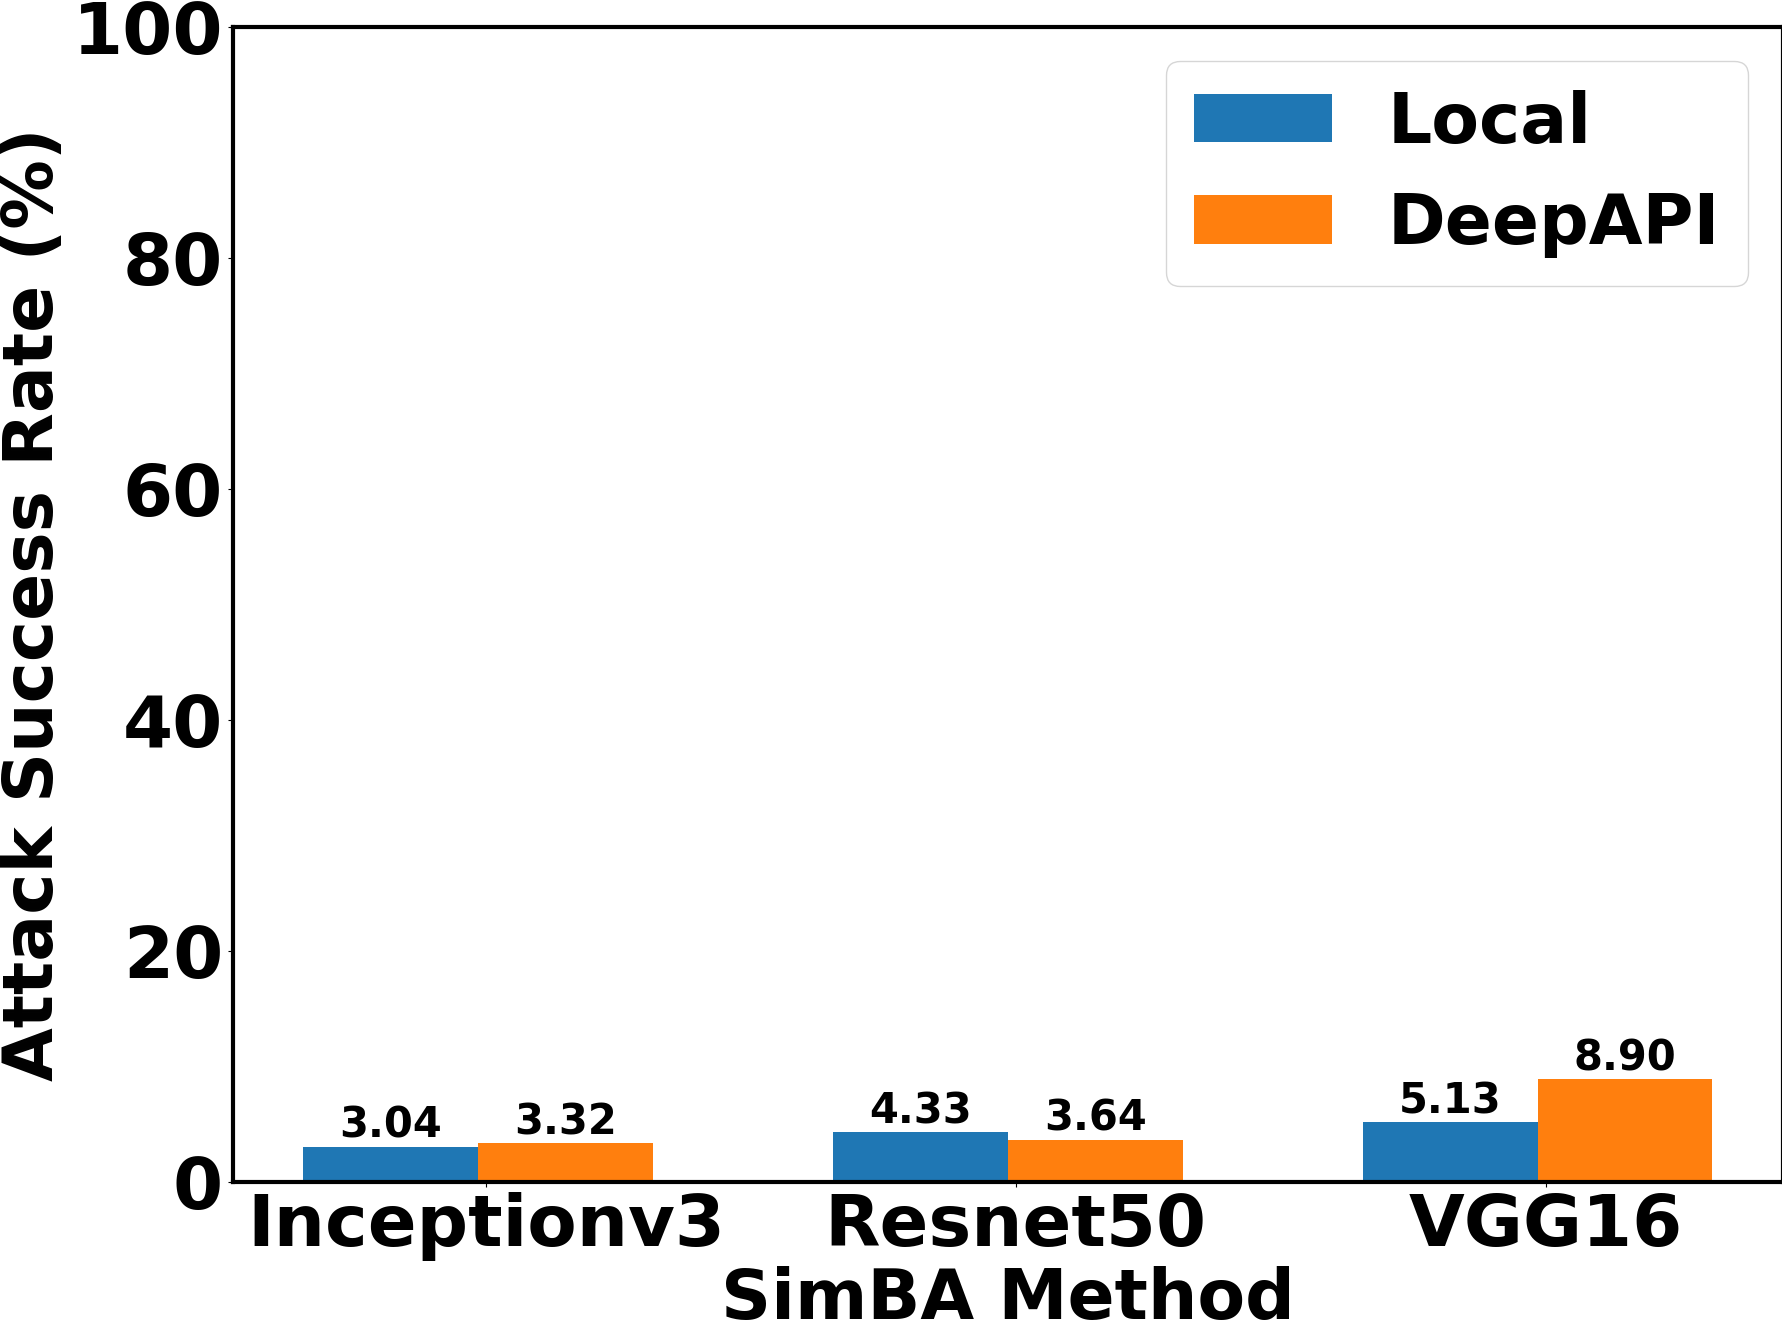
\includegraphics[width=\textwidth]{figures/chapter_classification/simba_attack_success_rate.png}
    \caption{SimBA (Baseline)}
    \label{fig:simba_suc}
\end{subfigure}
\hfill
\begin{subfigure}[b]{0.6\textwidth}
    \centering
    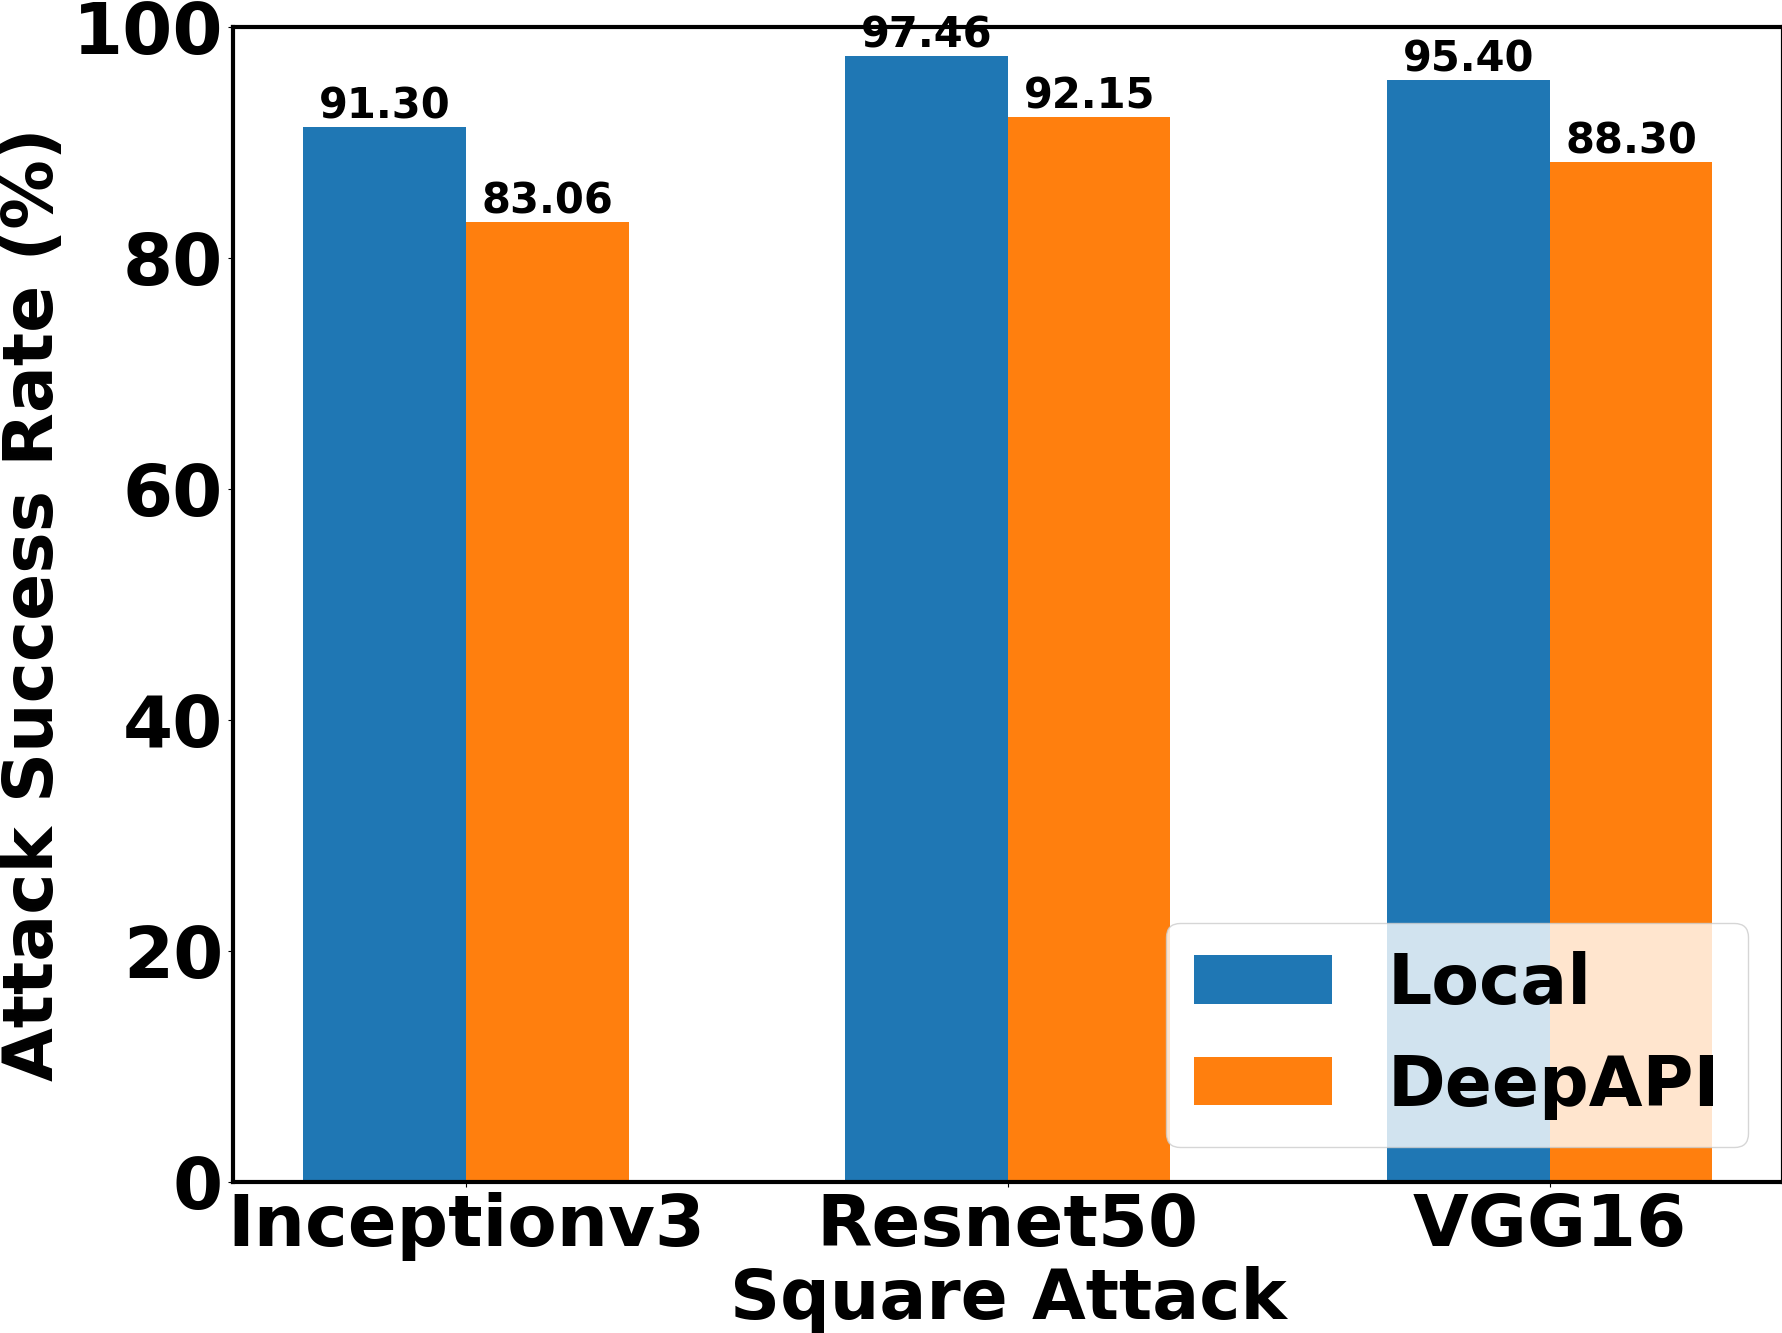
\includegraphics[width=\textwidth]{figures/chapter_classification/square_attack_success_rate.png}
    \caption{Square Attack (Local Search)}
    \label{fig:square_suc}
\end{subfigure}
\hfill
\begin{subfigure}[b]{0.6\textwidth}
    \centering
    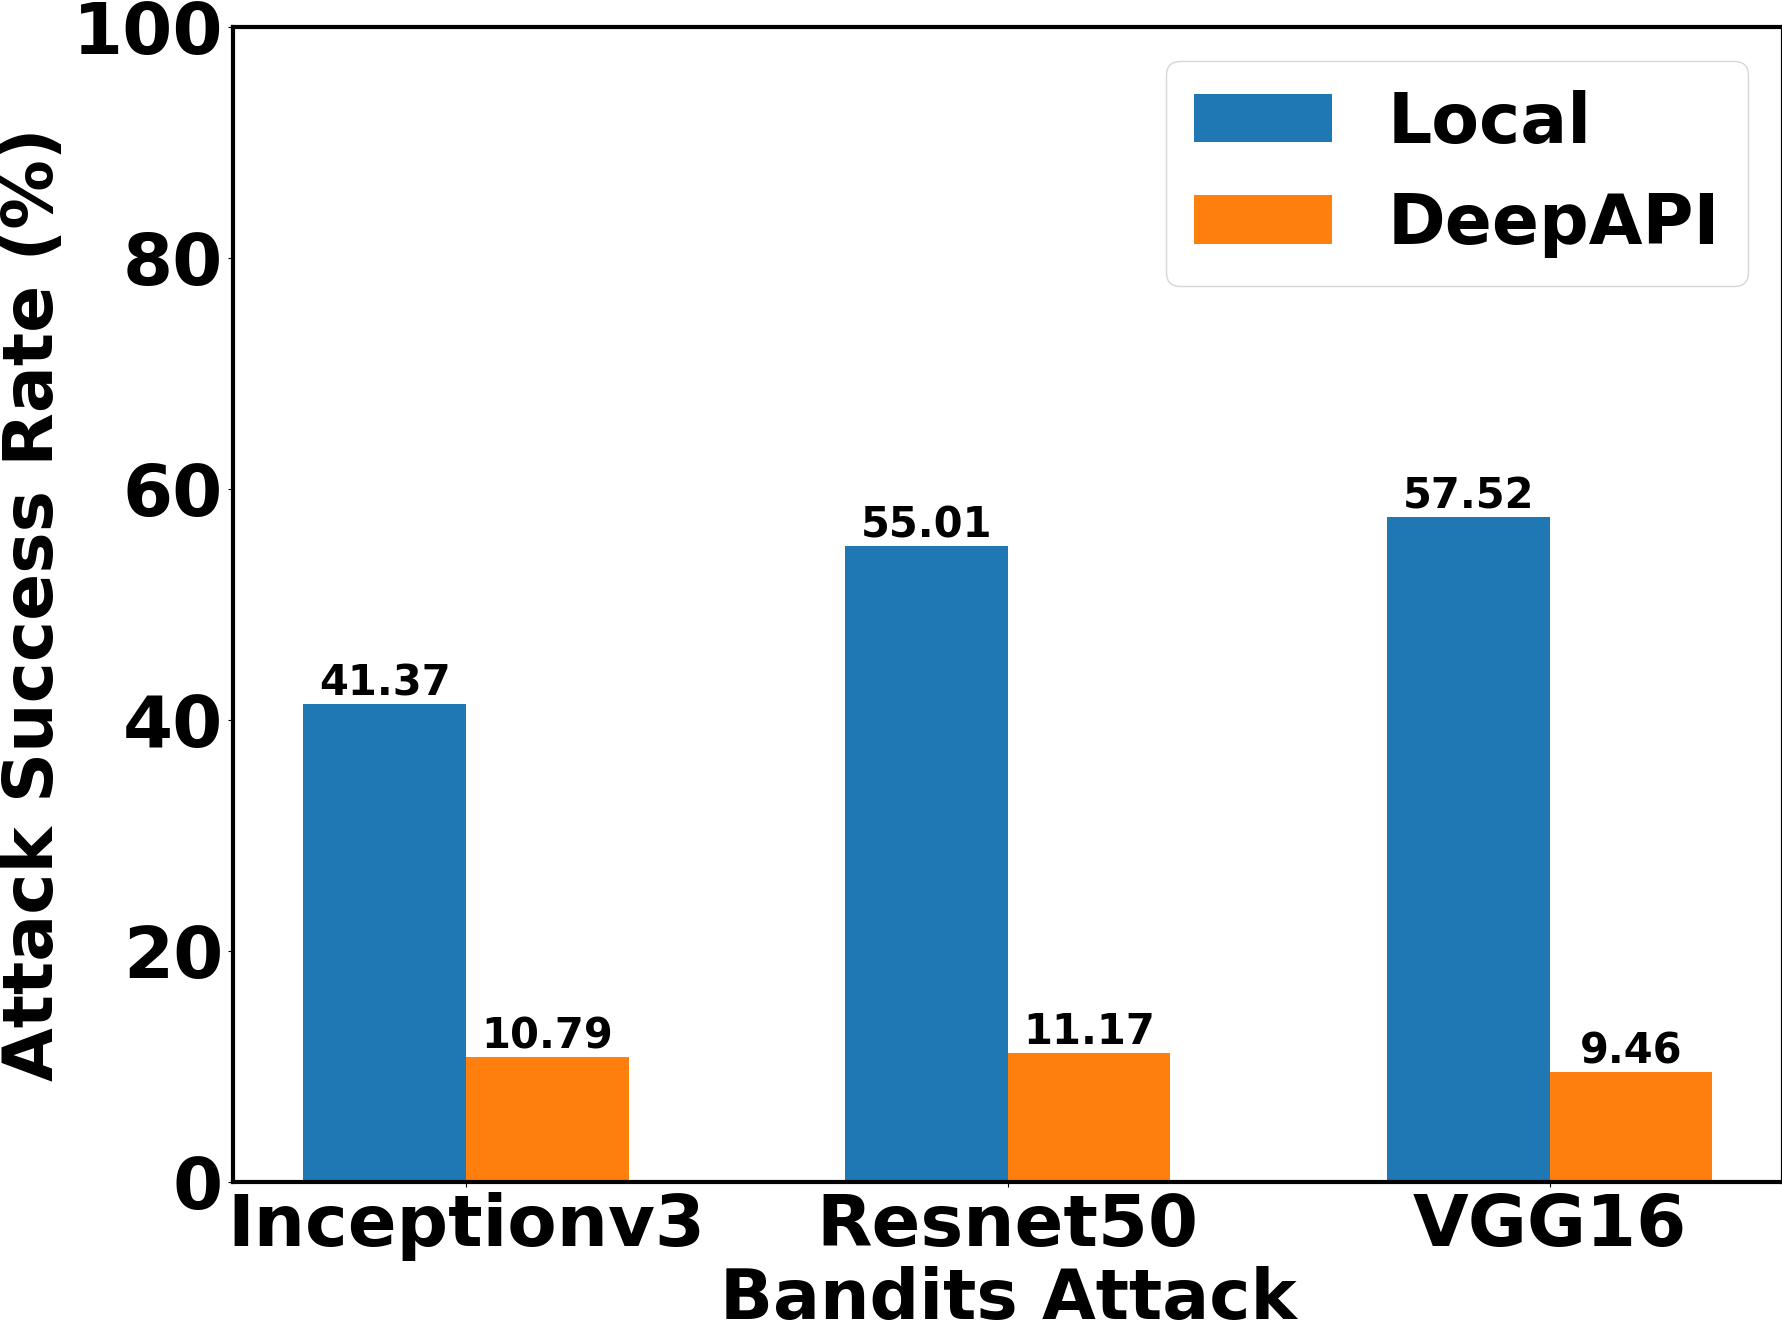
\includegraphics[width=\textwidth]{figures/chapter_classification/bandits_attack_success_rate.png}
    \caption{Bandits Attack (Gradient Estimation)}
    \label{fig:bandits_suc}
\end{subfigure}
\caption{The attack success rate tested on local models and cloud APIs.}
\label{fig.suc}
\end{figure*}

\begin{figure*}[tbp]
\centering
\begin{subfigure}[b]{0.6\textwidth}
    \centering
    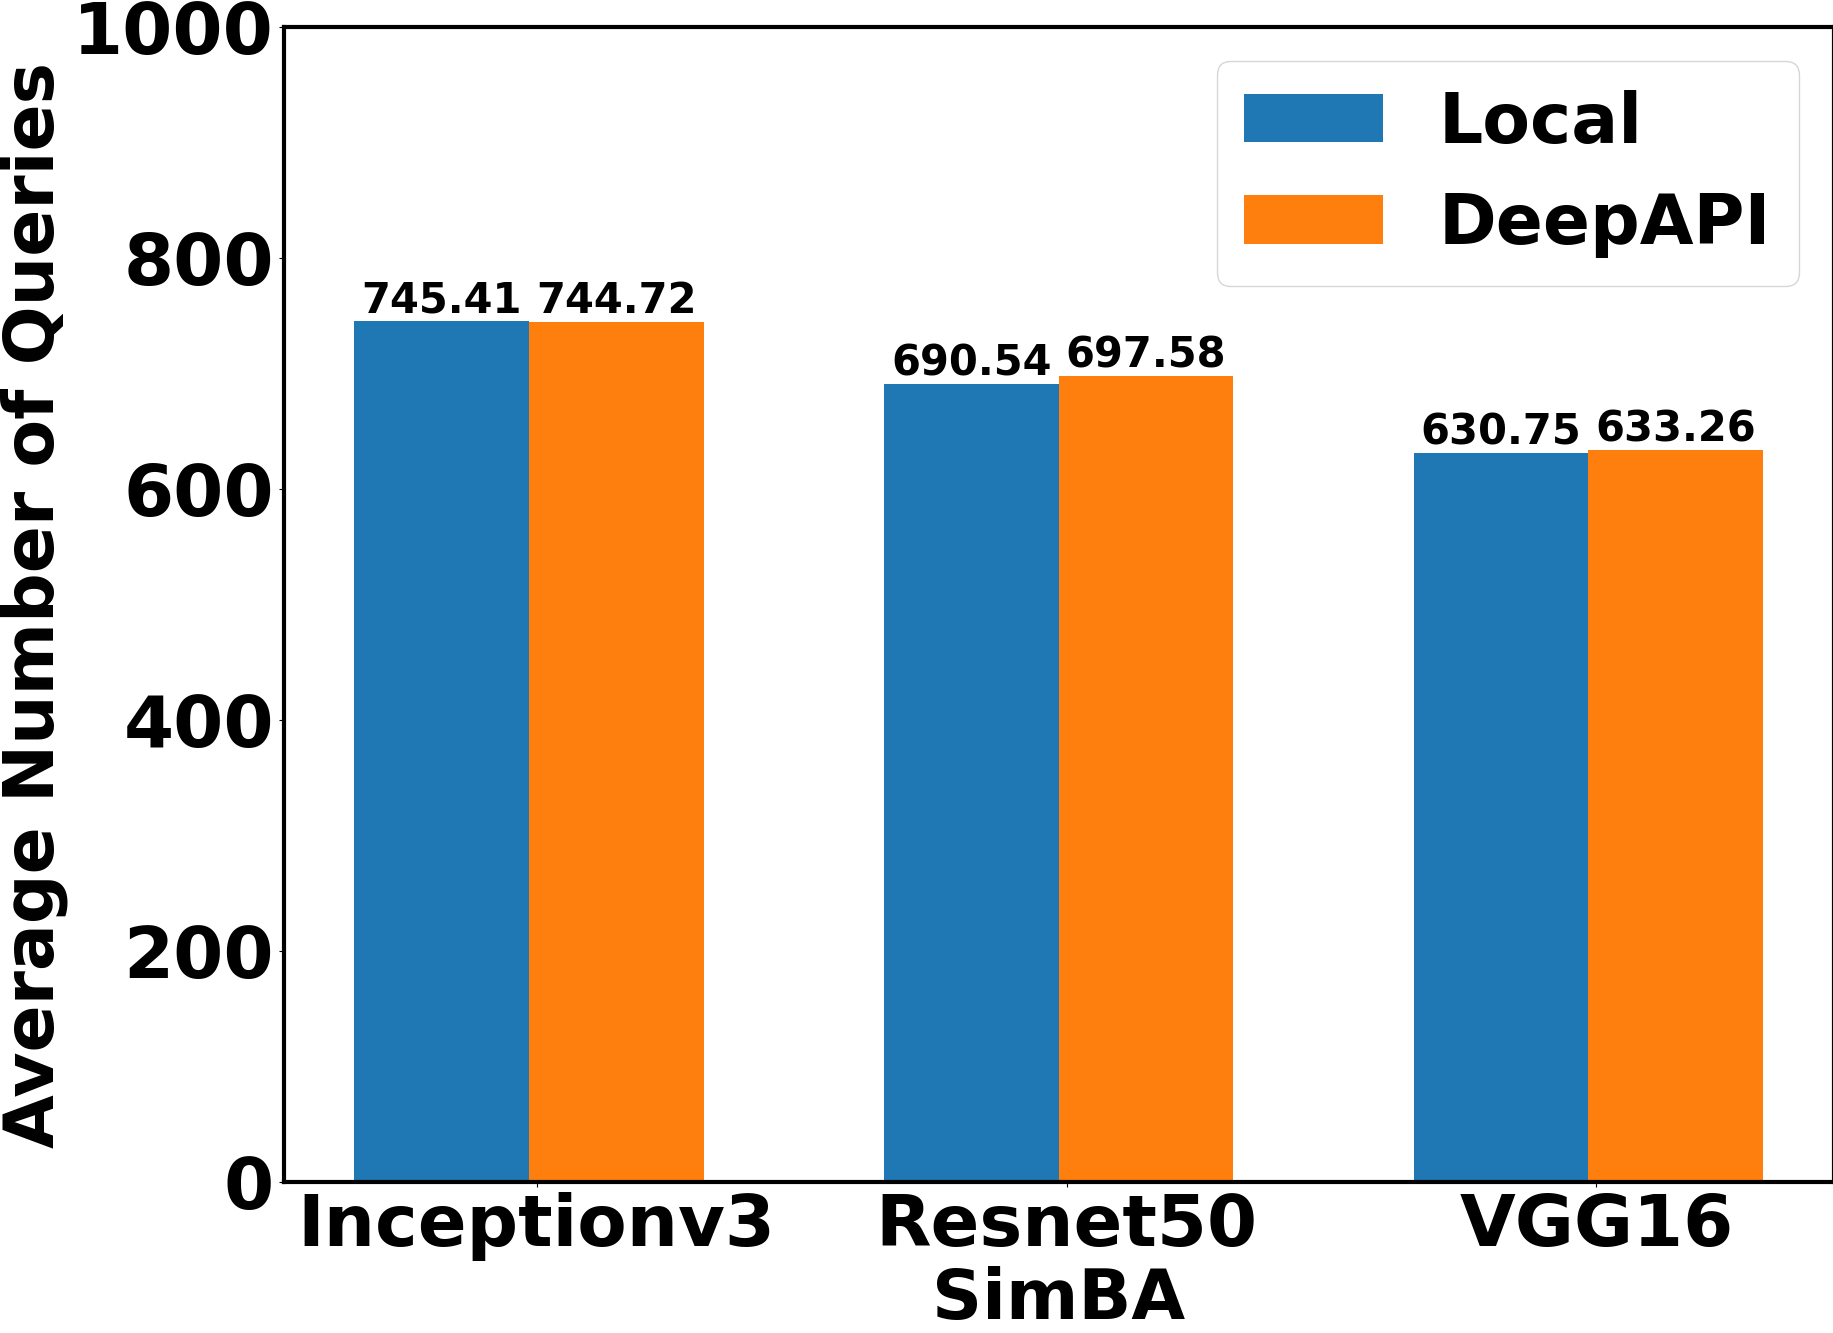
\includegraphics[width=\textwidth]{figures/chapter_classification/simba_number_of_queries.png}
    \caption{SimBA (Baseline)}
    \label{fig:simba_queries}
\end{subfigure}
\hfill
\begin{subfigure}[b]{0.6\textwidth}
    \centering
    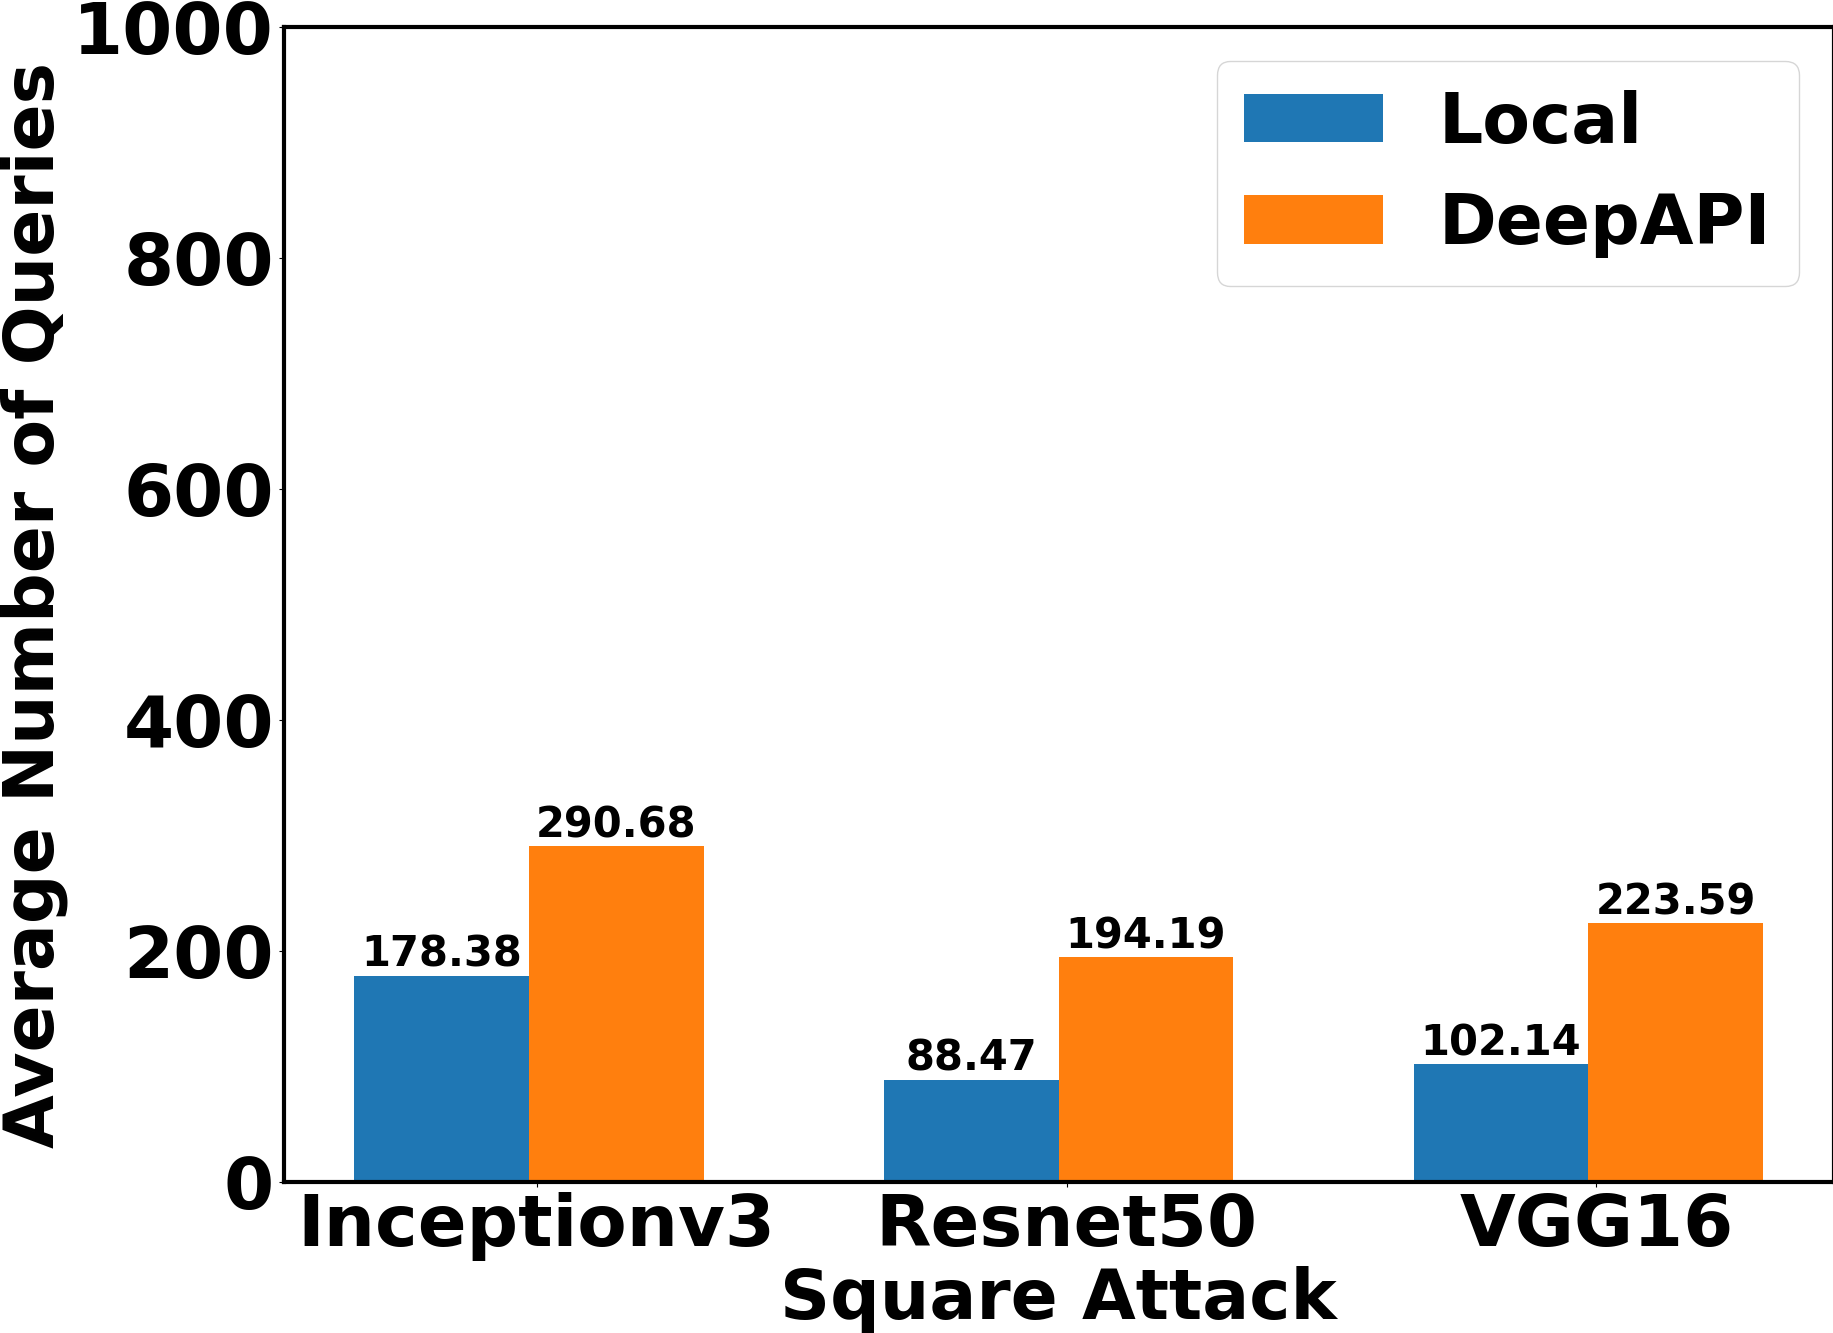
\includegraphics[width=\textwidth]{figures/chapter_classification/square_number_of_queries.png}
    \caption{Square Attack (Local Search)}
    \label{fig:square_queries}
\end{subfigure}
\hfill
\begin{subfigure}[b]{0.6\textwidth}
    \centering
    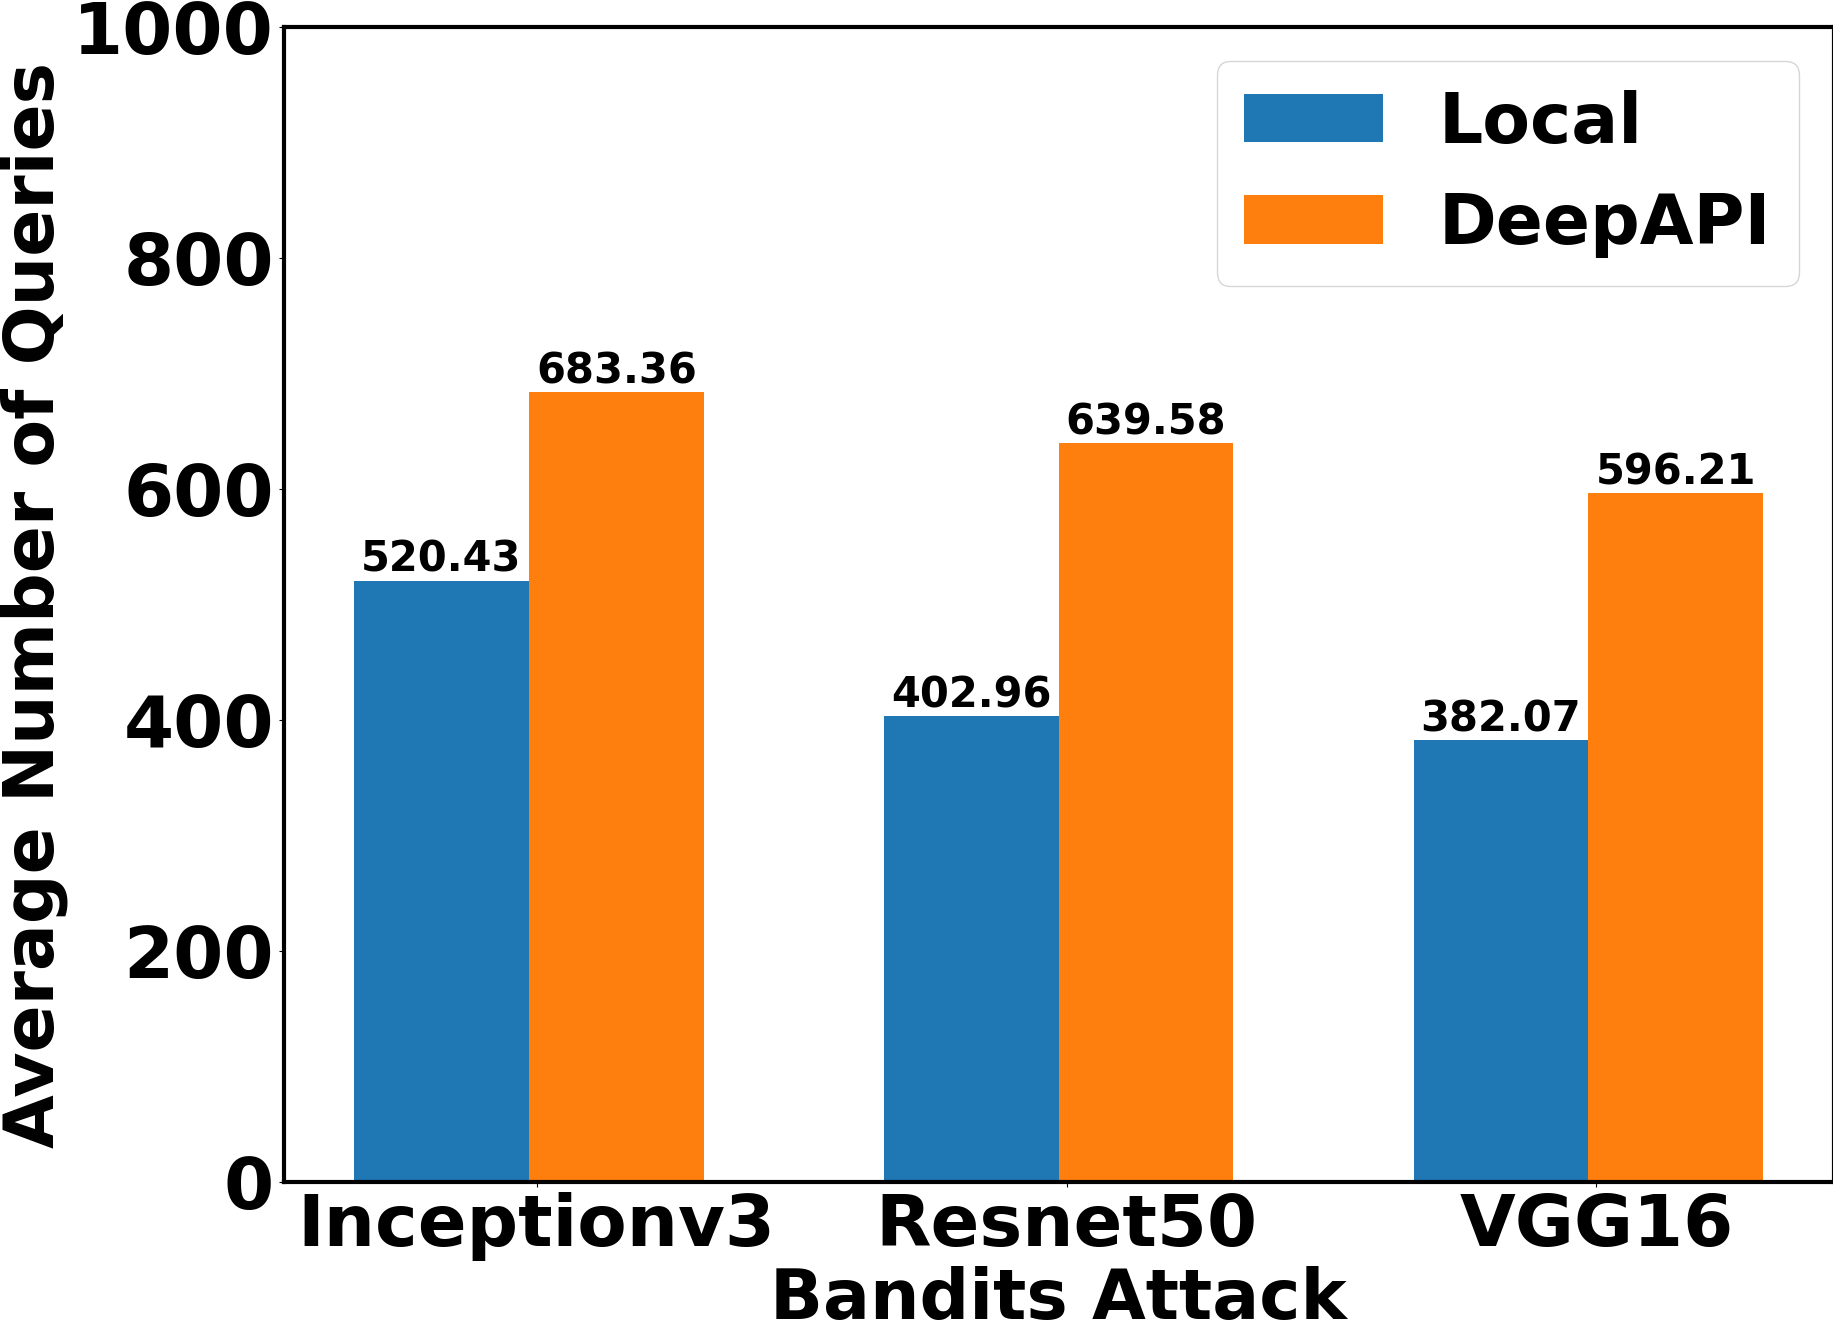
\includegraphics[width=\textwidth]{figures/chapter_classification/bandits_number_of_queries.png}
    \caption{Bandits Attack (Gradient Estimation)}
    \label{fig:bandits_queries}
\end{subfigure}
\caption{The average number of queries tested on local models and cloud APIs}
\label{fig.queries}
\end{figure*}

\begin{figure*}[tbp]
\centering
\begin{subfigure}[b]{0.6\textwidth}
    \centering
    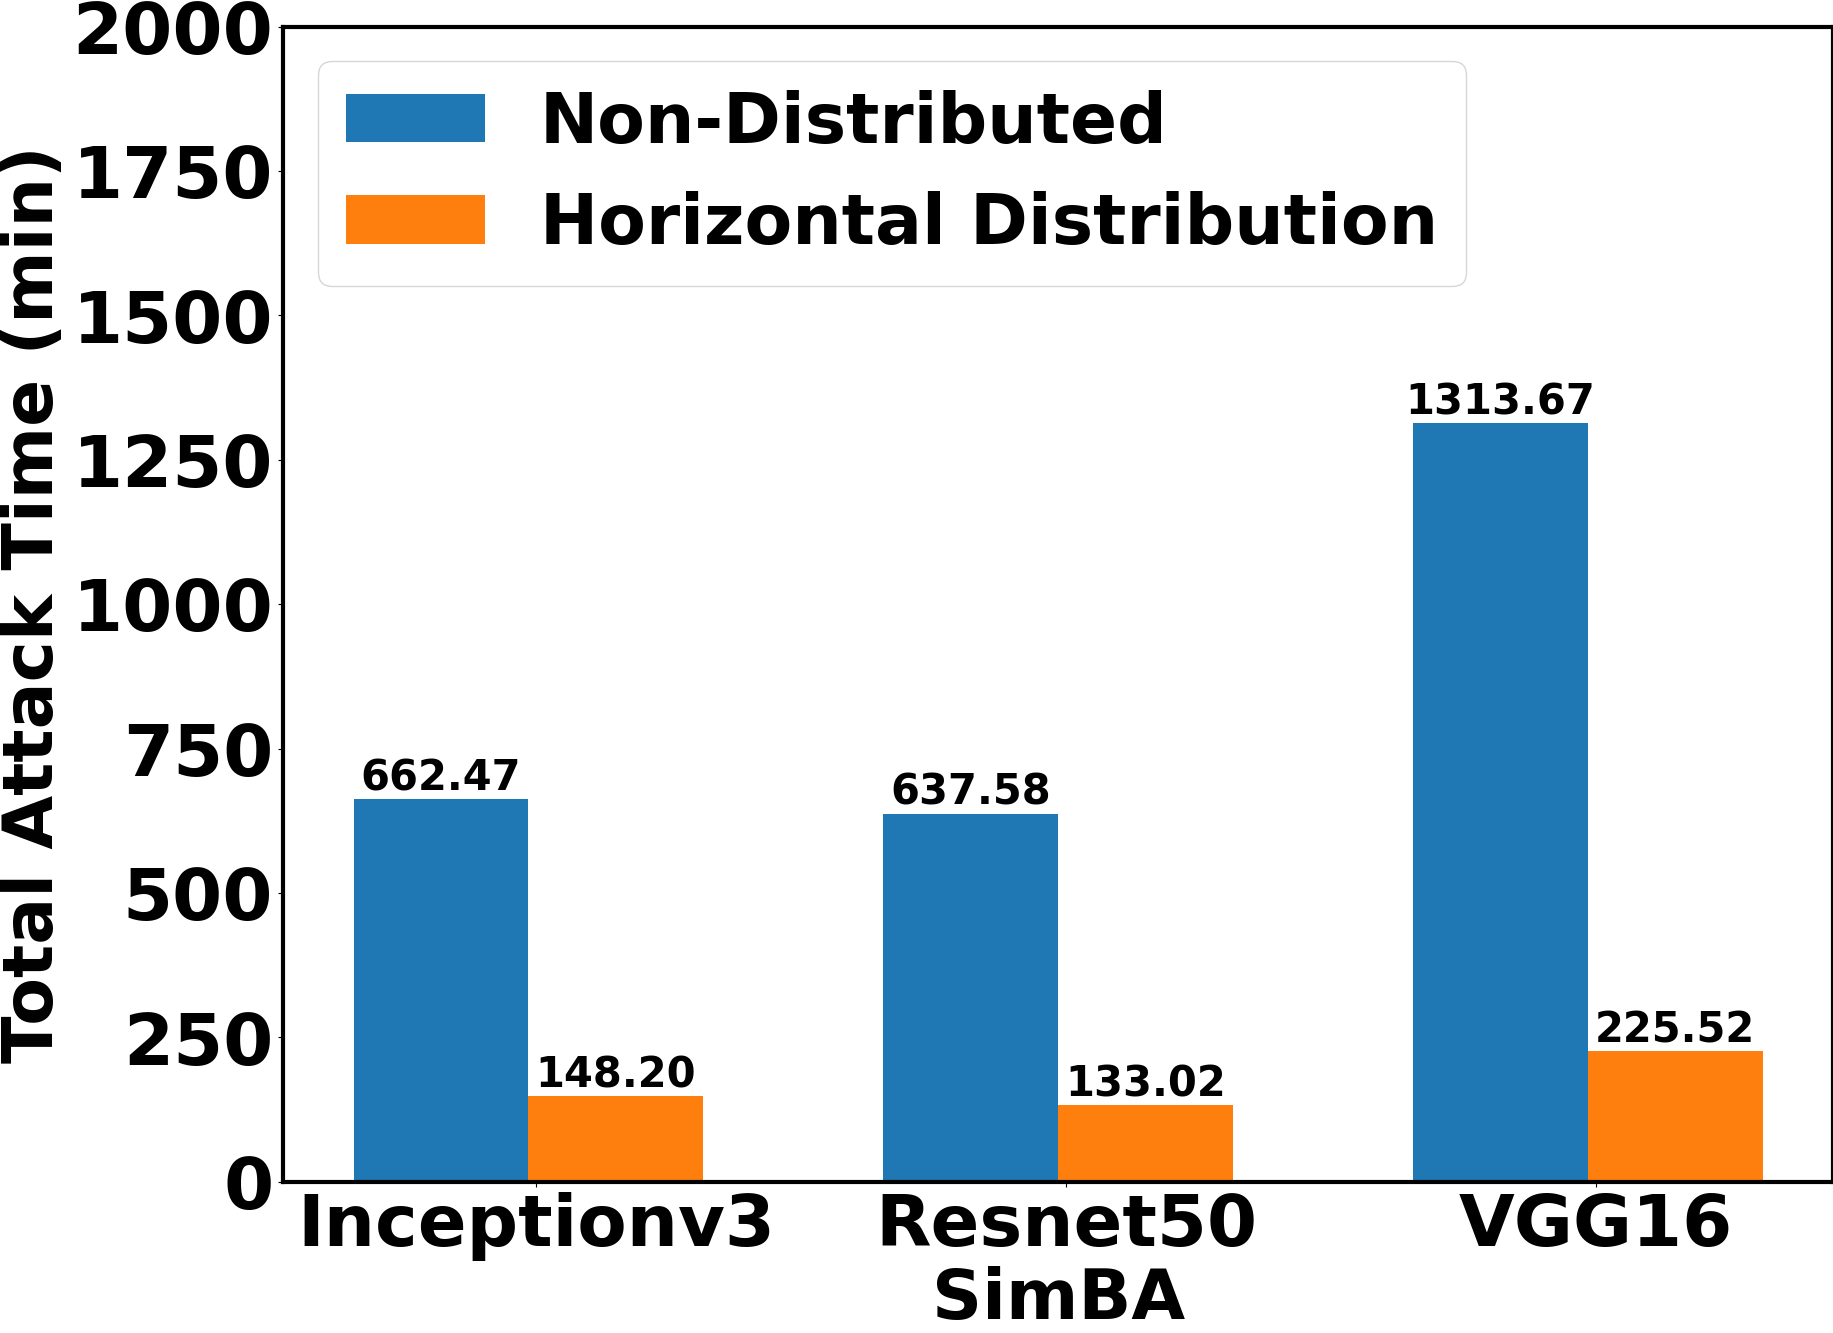
\includegraphics[width=\textwidth]{figures/chapter_classification/simba_attack_horizontal_time.png}
    \caption{SimBA (Baseline)}
    \label{fig:simba_horizon}
\end{subfigure}
\hfill
\begin{subfigure}[b]{0.6\textwidth}
    \centering
    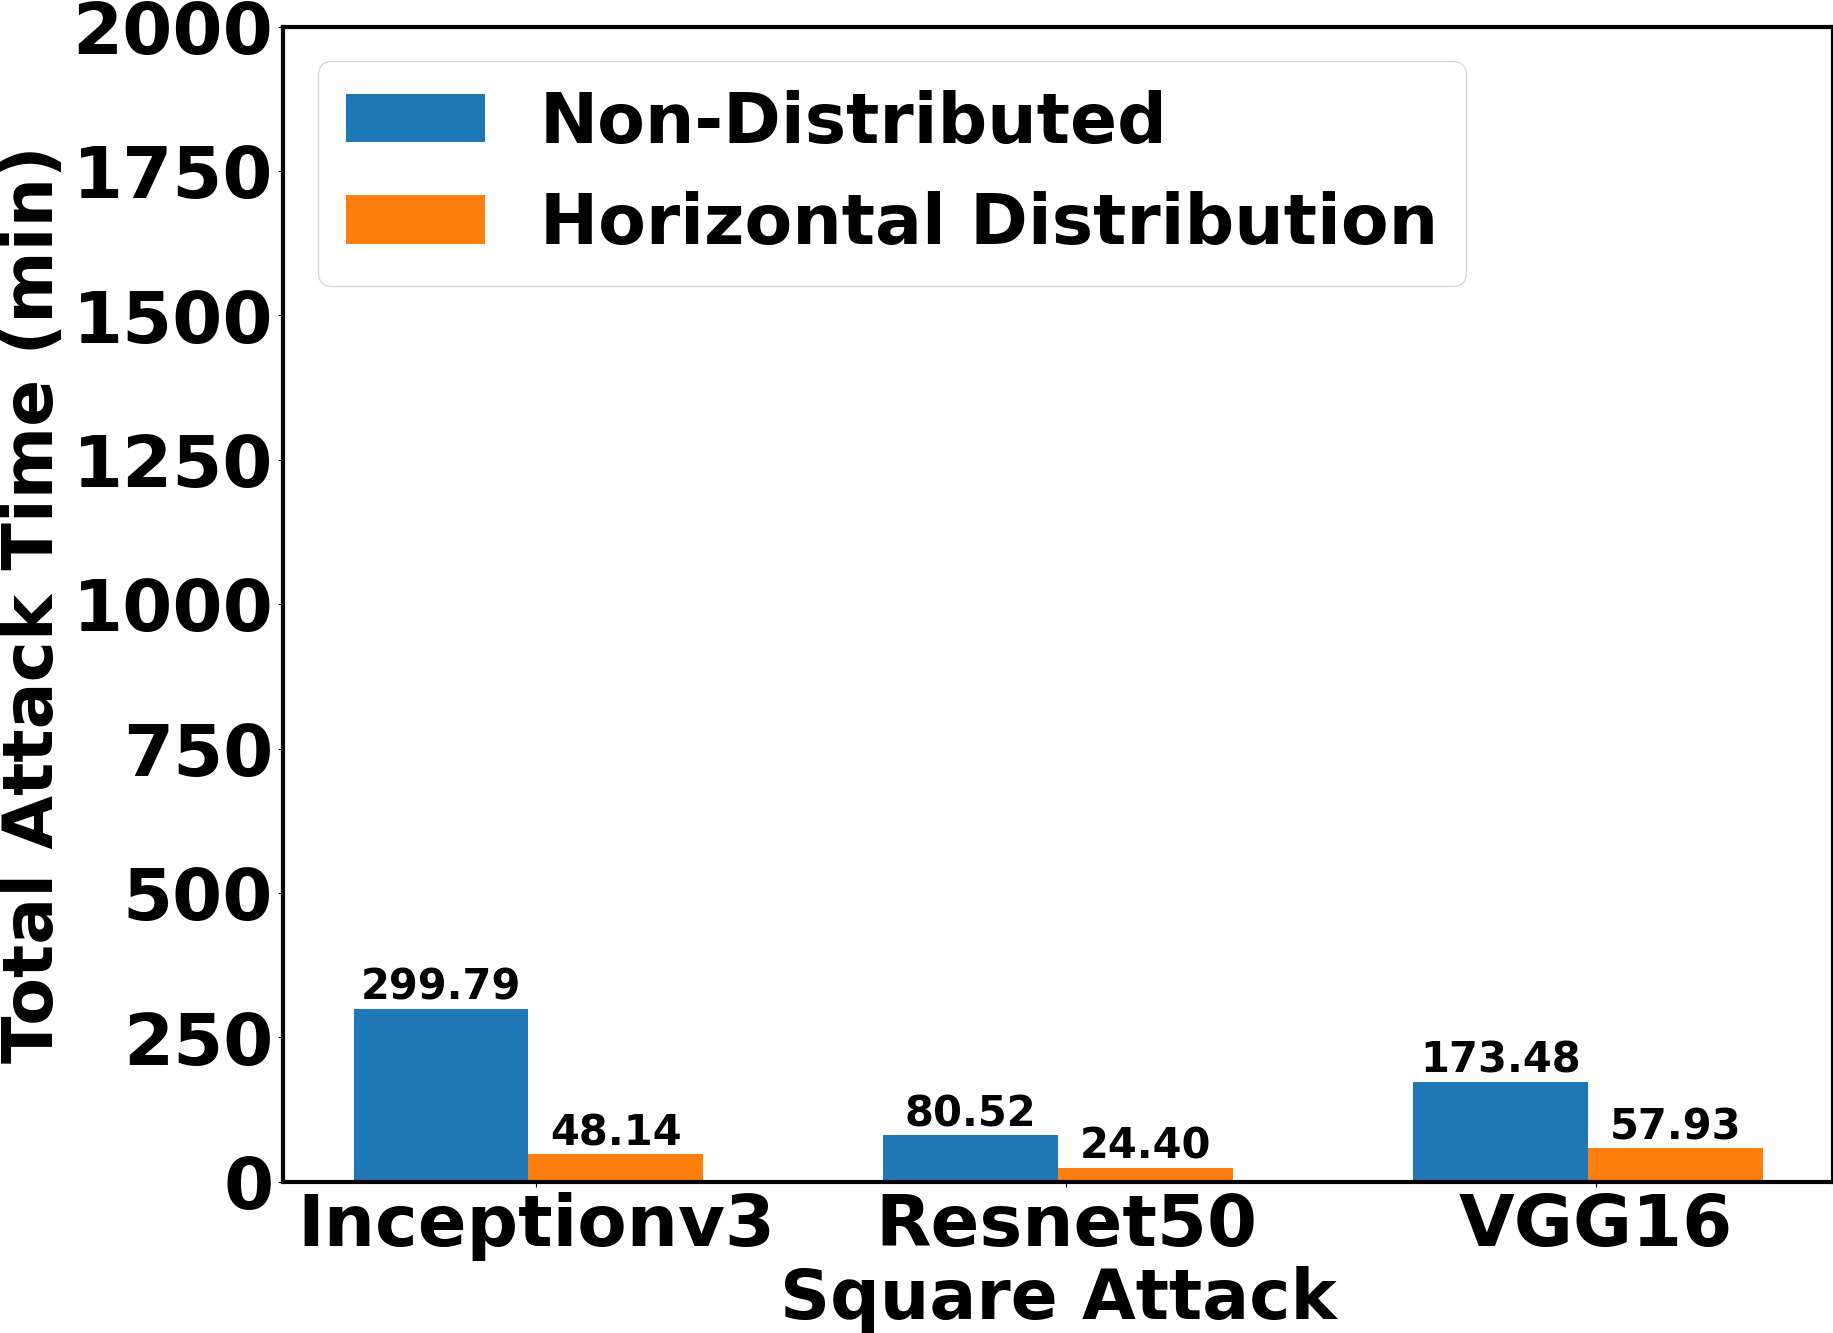
\includegraphics[width=\textwidth]{figures/chapter_classification/square_attack_horizontal_time.png}
    \caption{Square Attack (Local Search)}
    \label{fig:square_horizon}
\end{subfigure}
\hfill
\begin{subfigure}[b]{0.6\textwidth}
    \centering
    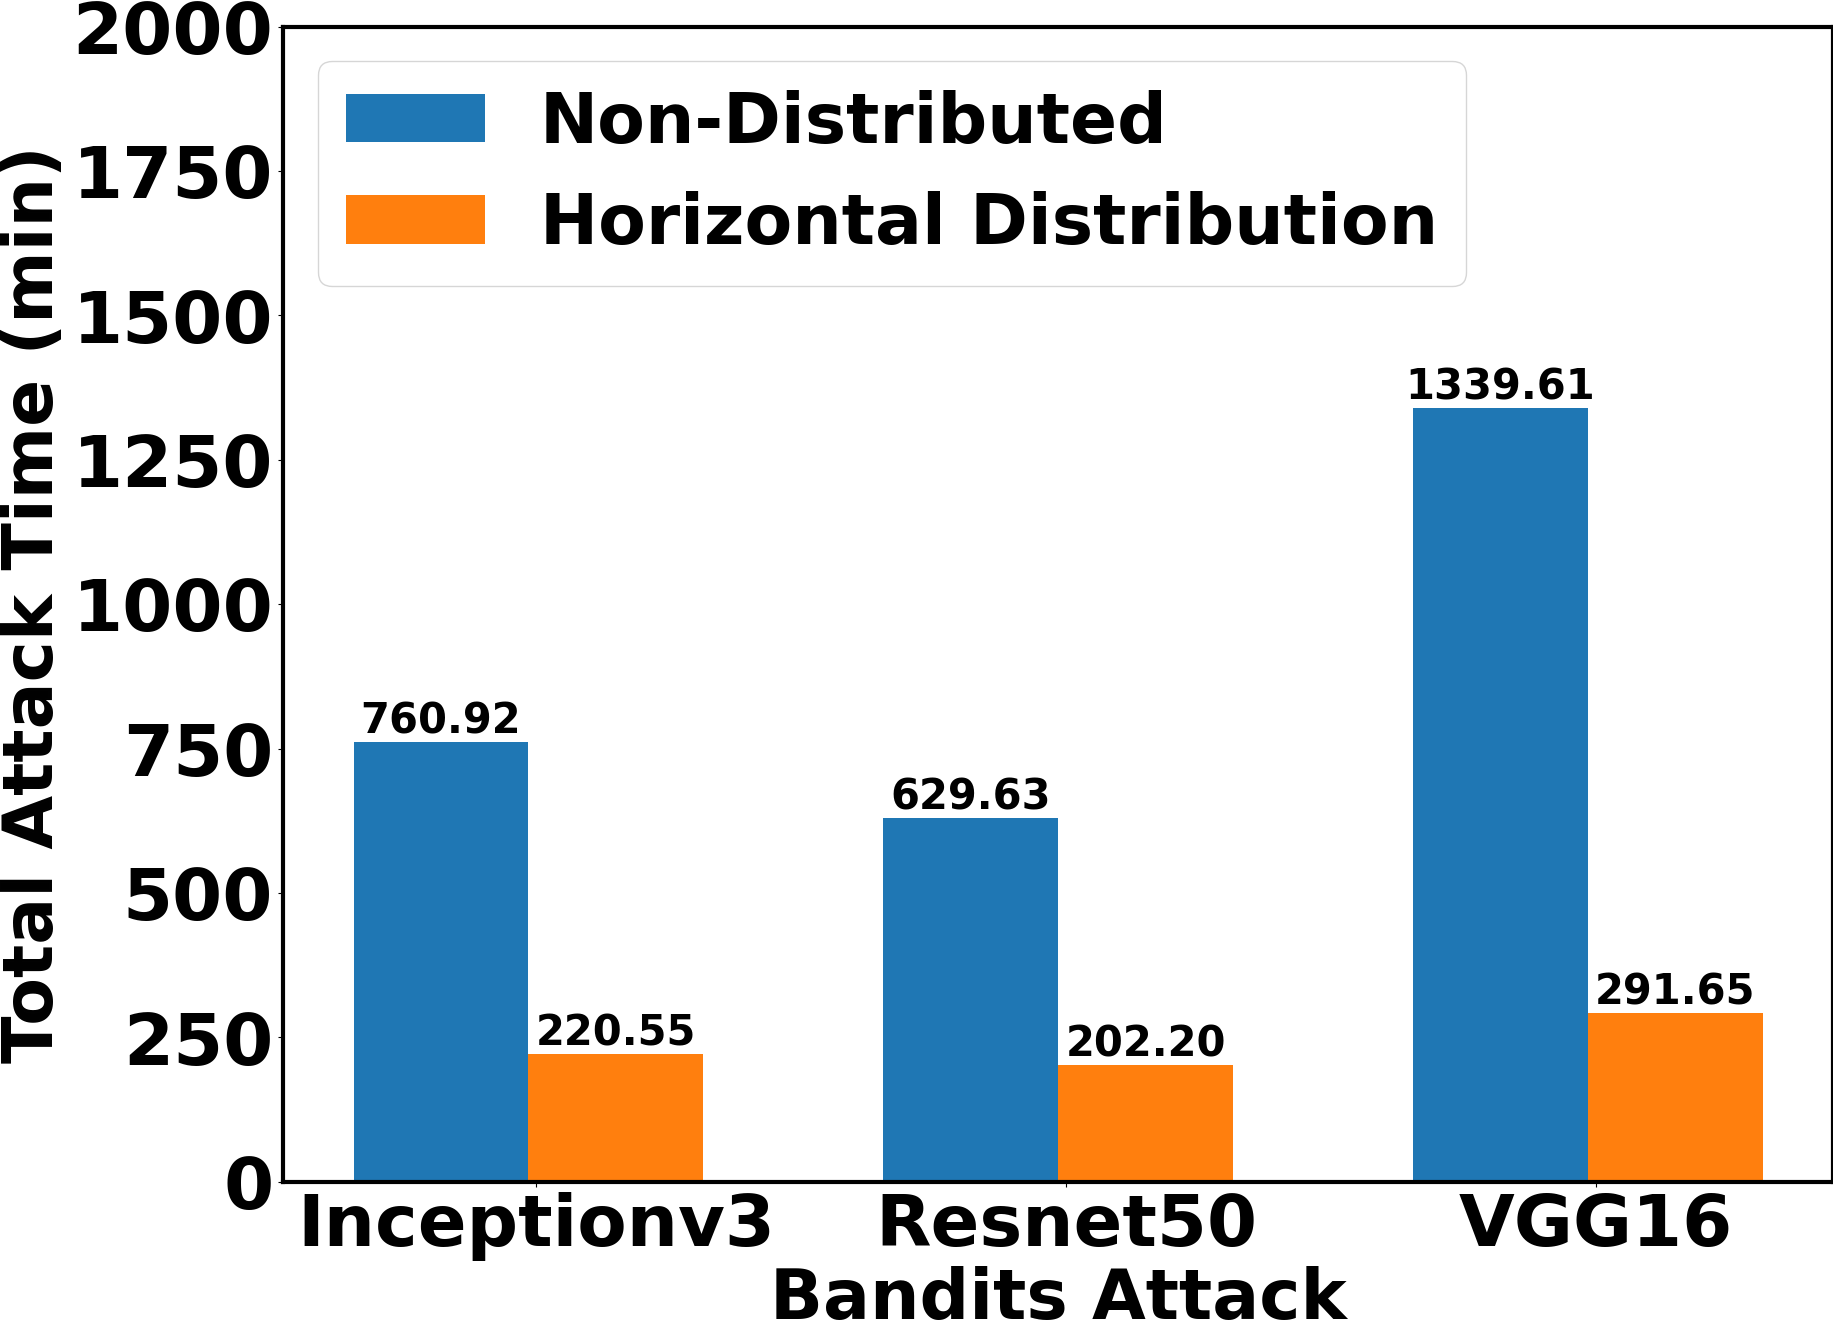
\includegraphics[width=\textwidth]{figures/chapter_classification/bandits_attack_horizontal_time.png}
    \caption{Bandits Attack (Gradient Estimation)}
    \label{fig:bandits_horizon}
\end{subfigure}
\caption{The total attack time with and without horizontal distribution.}
\label{fig.horizon_time}
\end{figure*}

\clearpage

\subsection{Vertical Distribution}

In this section, we focus on improving the efficiency of attacking a single image through vertical distribution, which sends out queries concurrently across iterations of an image. 

In the following experiments, we use the implementation presented in Section \ref{horizon_vertical}. The implementations of vertical distribution presented in Section \ref{horizon_vertical} serve to illustrate the general concept of distributed attacks, but there may be other approaches to achieving vertical distribution that are more effective for a specific black-box attack.

% In this section, we focus on improving the iteration process for attacking a single image using vertical distribution. The vertical distribution accelerates the attack by concurrently sending out queries across iterations of the same image. In the following experiments, We use examples of vertical distribution illustrated in Section \ref{horizon_vertical}, while there are different ways to achieve vertical distribution for a specific black-box attack.

\textbf{The SimBA Attack}: Though the baseline method, SimBA, achieves a relatively low attack success rate, we can use vertical distribution to accelerate the attack. Using vertical distribution, we randomly choose a batch of unrepeated pixels to perturb and the probability of the correct class decreases faster than the original non-distributed attack (see Fig. \ref{fig:simba_plot}). This is particularly effective when attacking with SimBA, which has a relatively low attack success rate. 

% Though the baseline method, SimBA, achieves a relatively low attack success rate, we can use vertical distribution to decrease the probability of the correct class faster until the model makes a wrong prediction. 

\textbf{The Square Attack}: Similarly, the vertically distributed square attack decreases the margin loss faster than the original method and achieves an early successful attack (see Fig. \ref{fig:square_plot}). This is because multiple square-shaped perturbations are generated as a batch in a single iteration.

\textbf{The Bandits Attack}: The vertically distributed bandits attack also achieves an early successful attack (see Fig. \ref{fig:bandits_plot}) by averaging a batch of concurrent gradient estimations, and thus improving the imperfect gradient estimator $\nabla_i$. Note that the original non-distributed Bandits Attack failed to generate an adversarial example after 1,000 queries, which means vertical distribution can also improve the attack success rate.

Besides, we show some adversarial images generated by vertically distributed black-box attacks and original methods (no vertical distribution) in Fig. \ref{fig.vertical_img}. They were generated under the same $\epsilon=0.05$, and we cannot tell the difference between images generated with and without vertical distribution from the perspective of human eyes.

In conclusion, compared with non-distributed attacks, vertically distributed attacks require less time to achieve a successful attack for each image, while the generated adversarial example is visually the same as in the original method. This highlights the potential of vertical distribution as an effective strategy for improving the efficiency of black-box attacks.


\begin{figure*}[tp]
\centering
\begin{subfigure}[b]{0.6\textwidth}
    \centering
    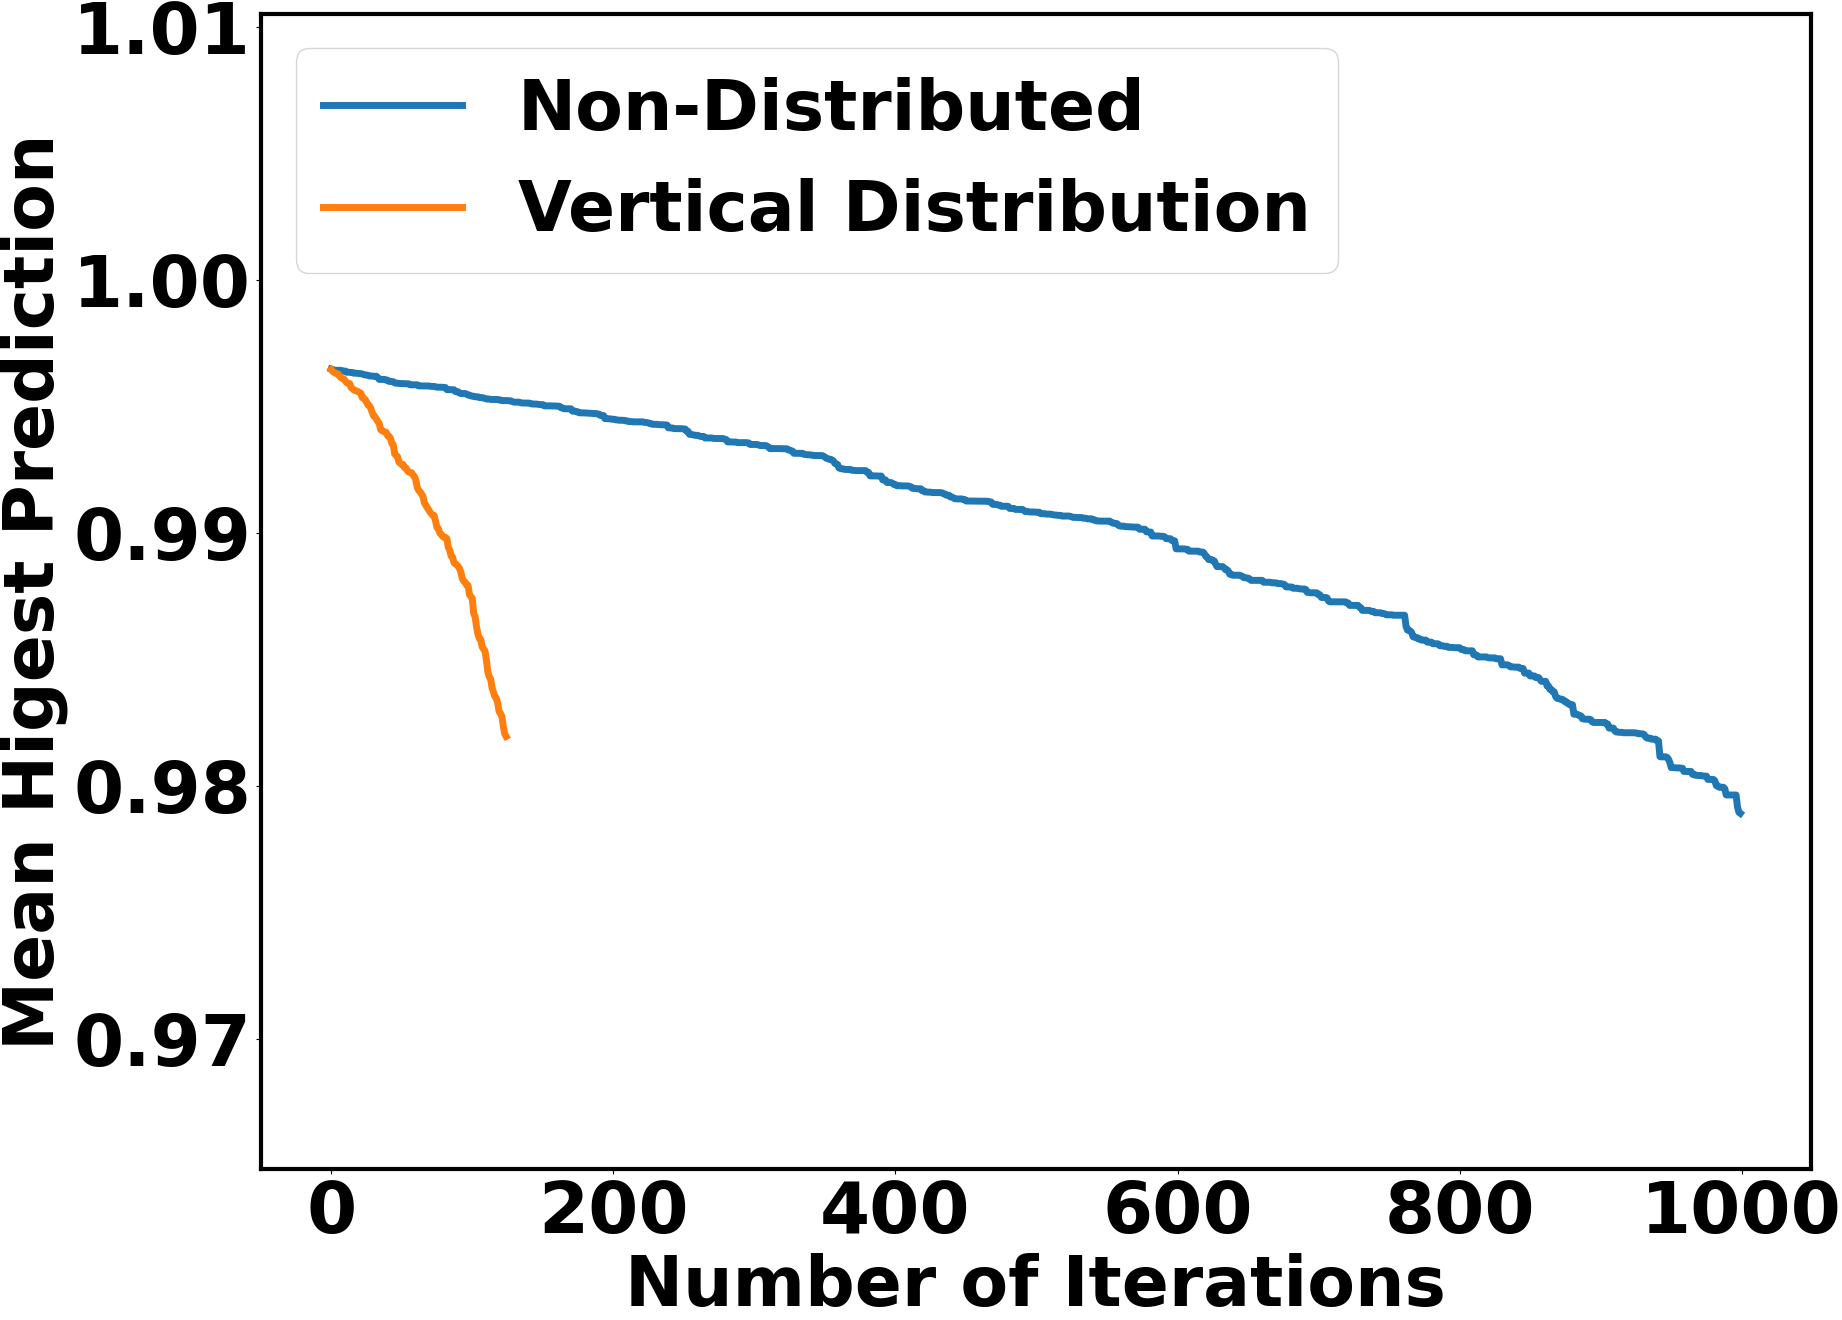
\includegraphics[width=\textwidth]{figures/chapter_classification/simba_attack_vertical_margin.png}
    \caption{SimBA (Baseline)}
    \label{fig:simba_plot}
\end{subfigure}
\hfill
\begin{subfigure}[b]{0.6\textwidth}
    \centering
    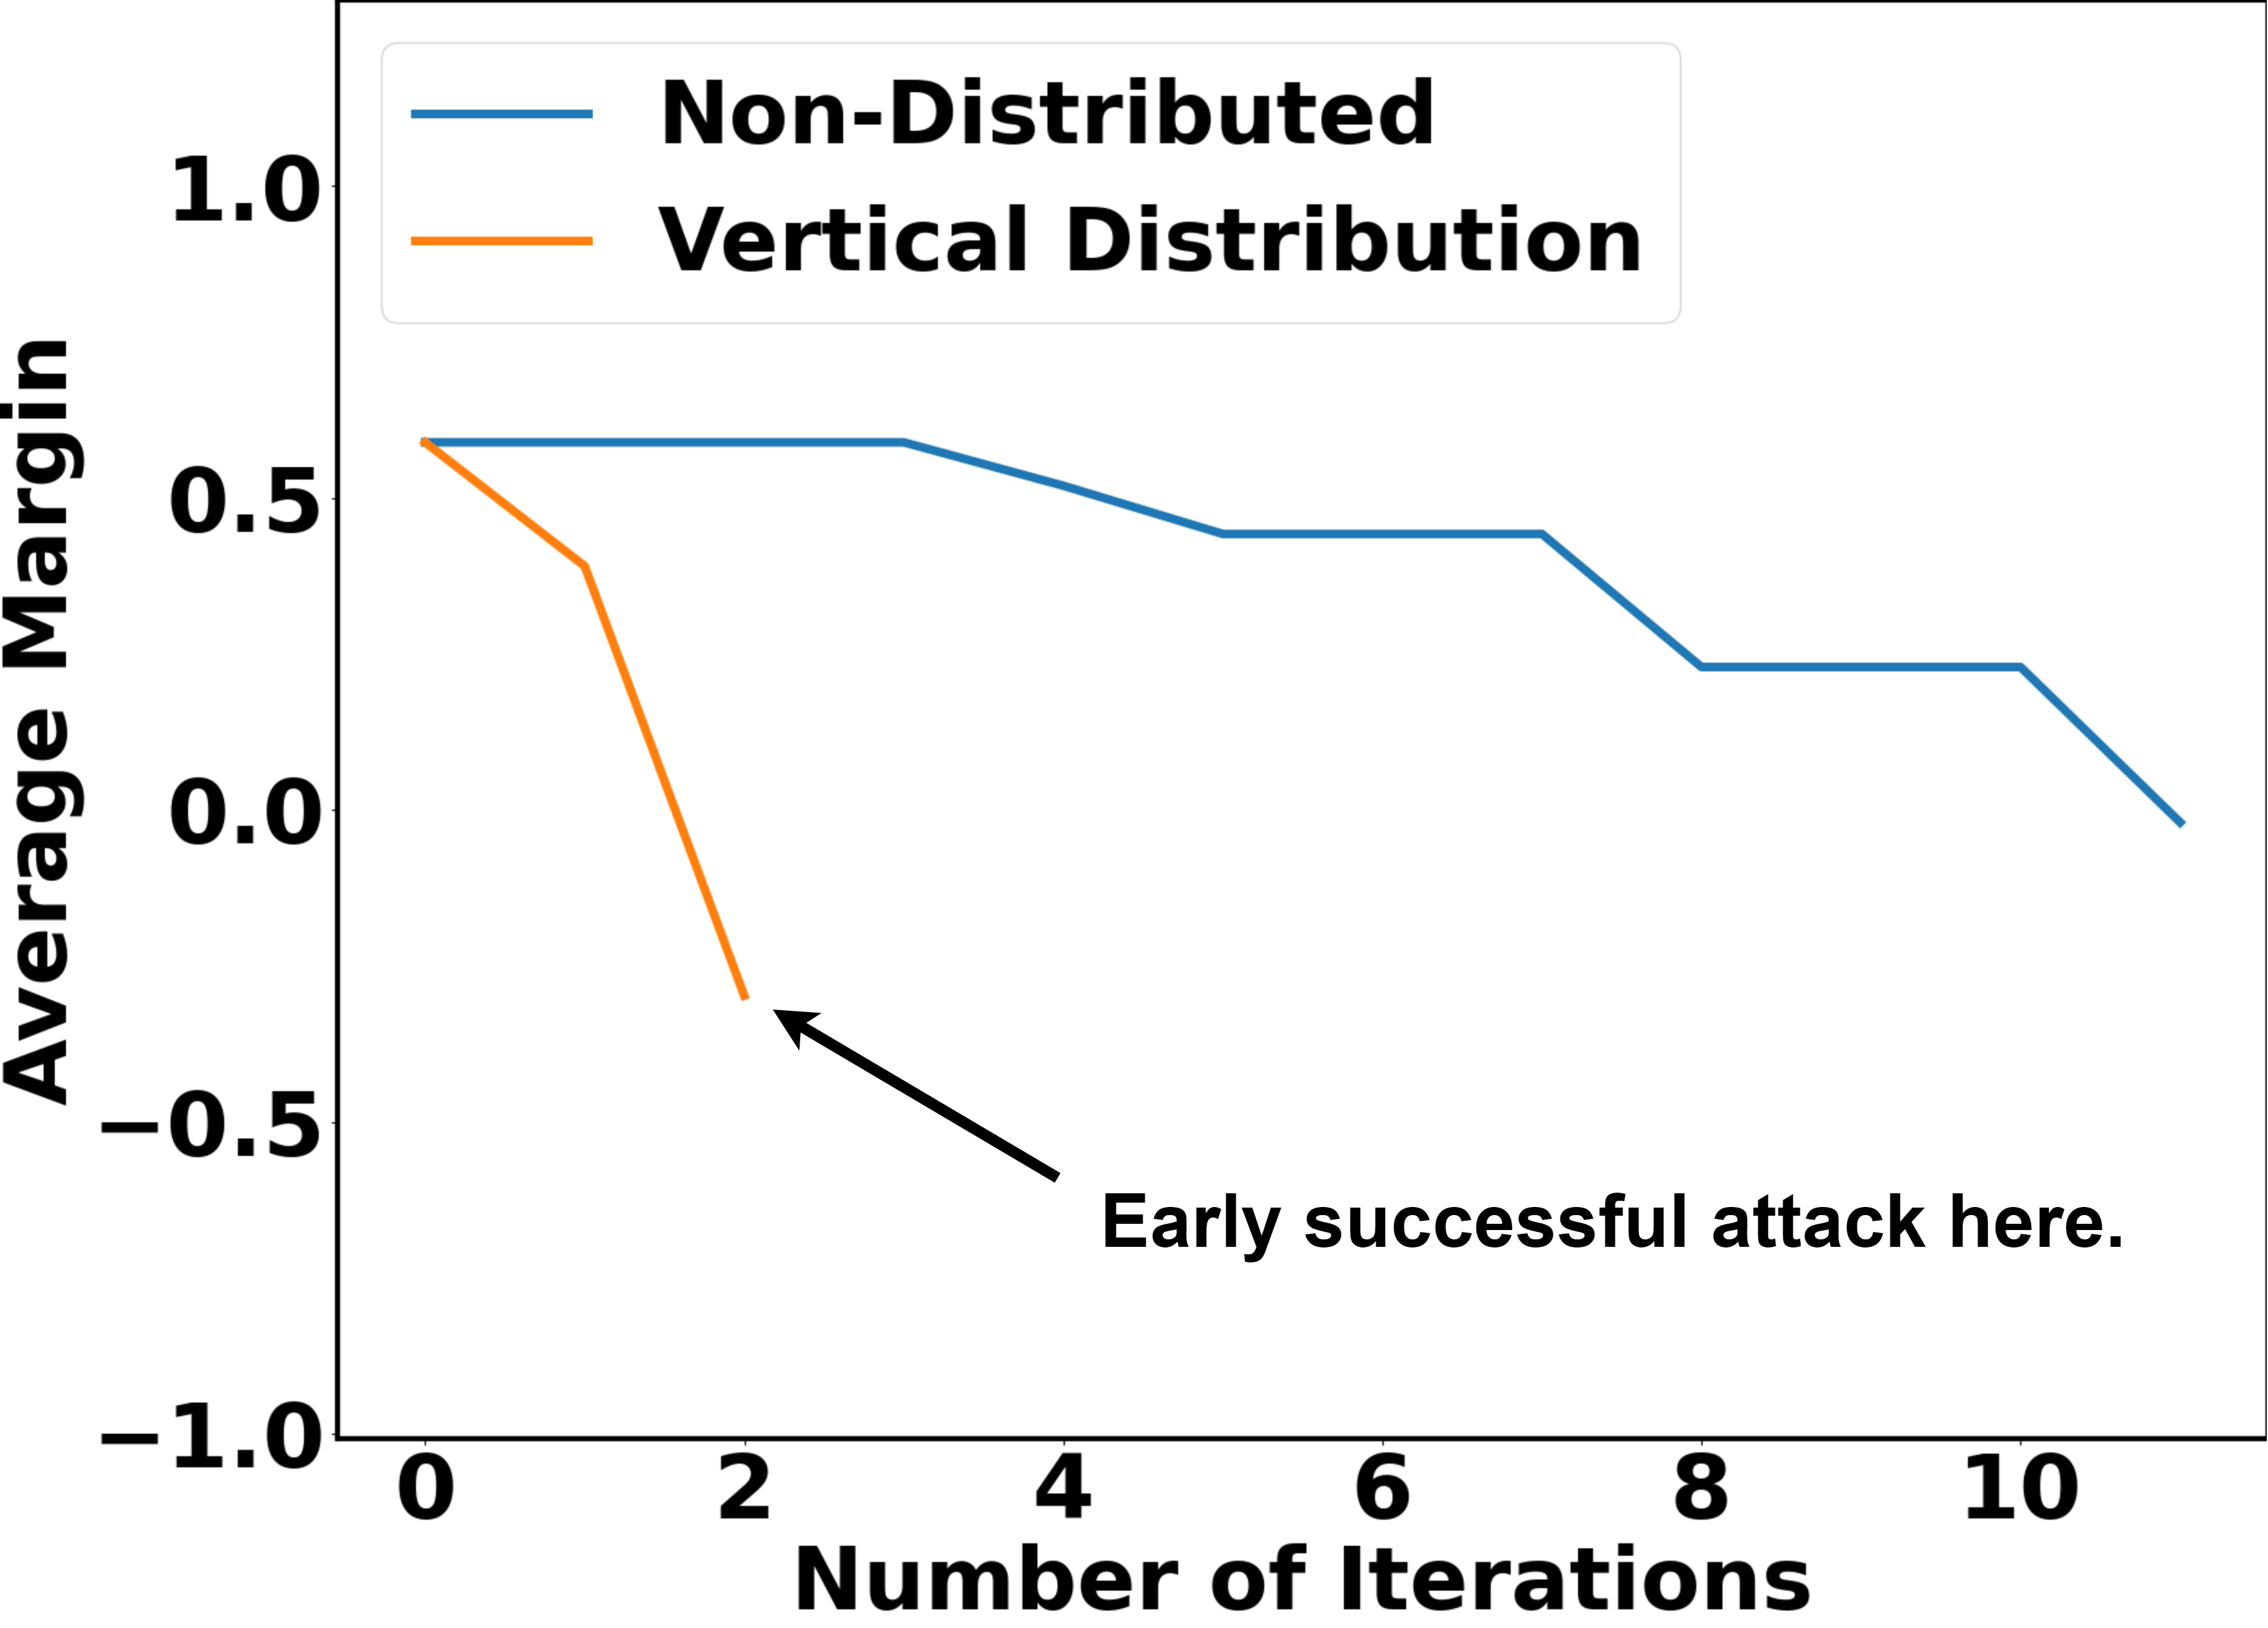
\includegraphics[width=\textwidth]{figures/chapter_classification/square_attack_vertical_margin.png}
    \caption{Square Attack (Local Search)}
    \label{fig:square_plot}
\end{subfigure}
\hfill
\begin{subfigure}[b]{0.6\textwidth}
    \centering
    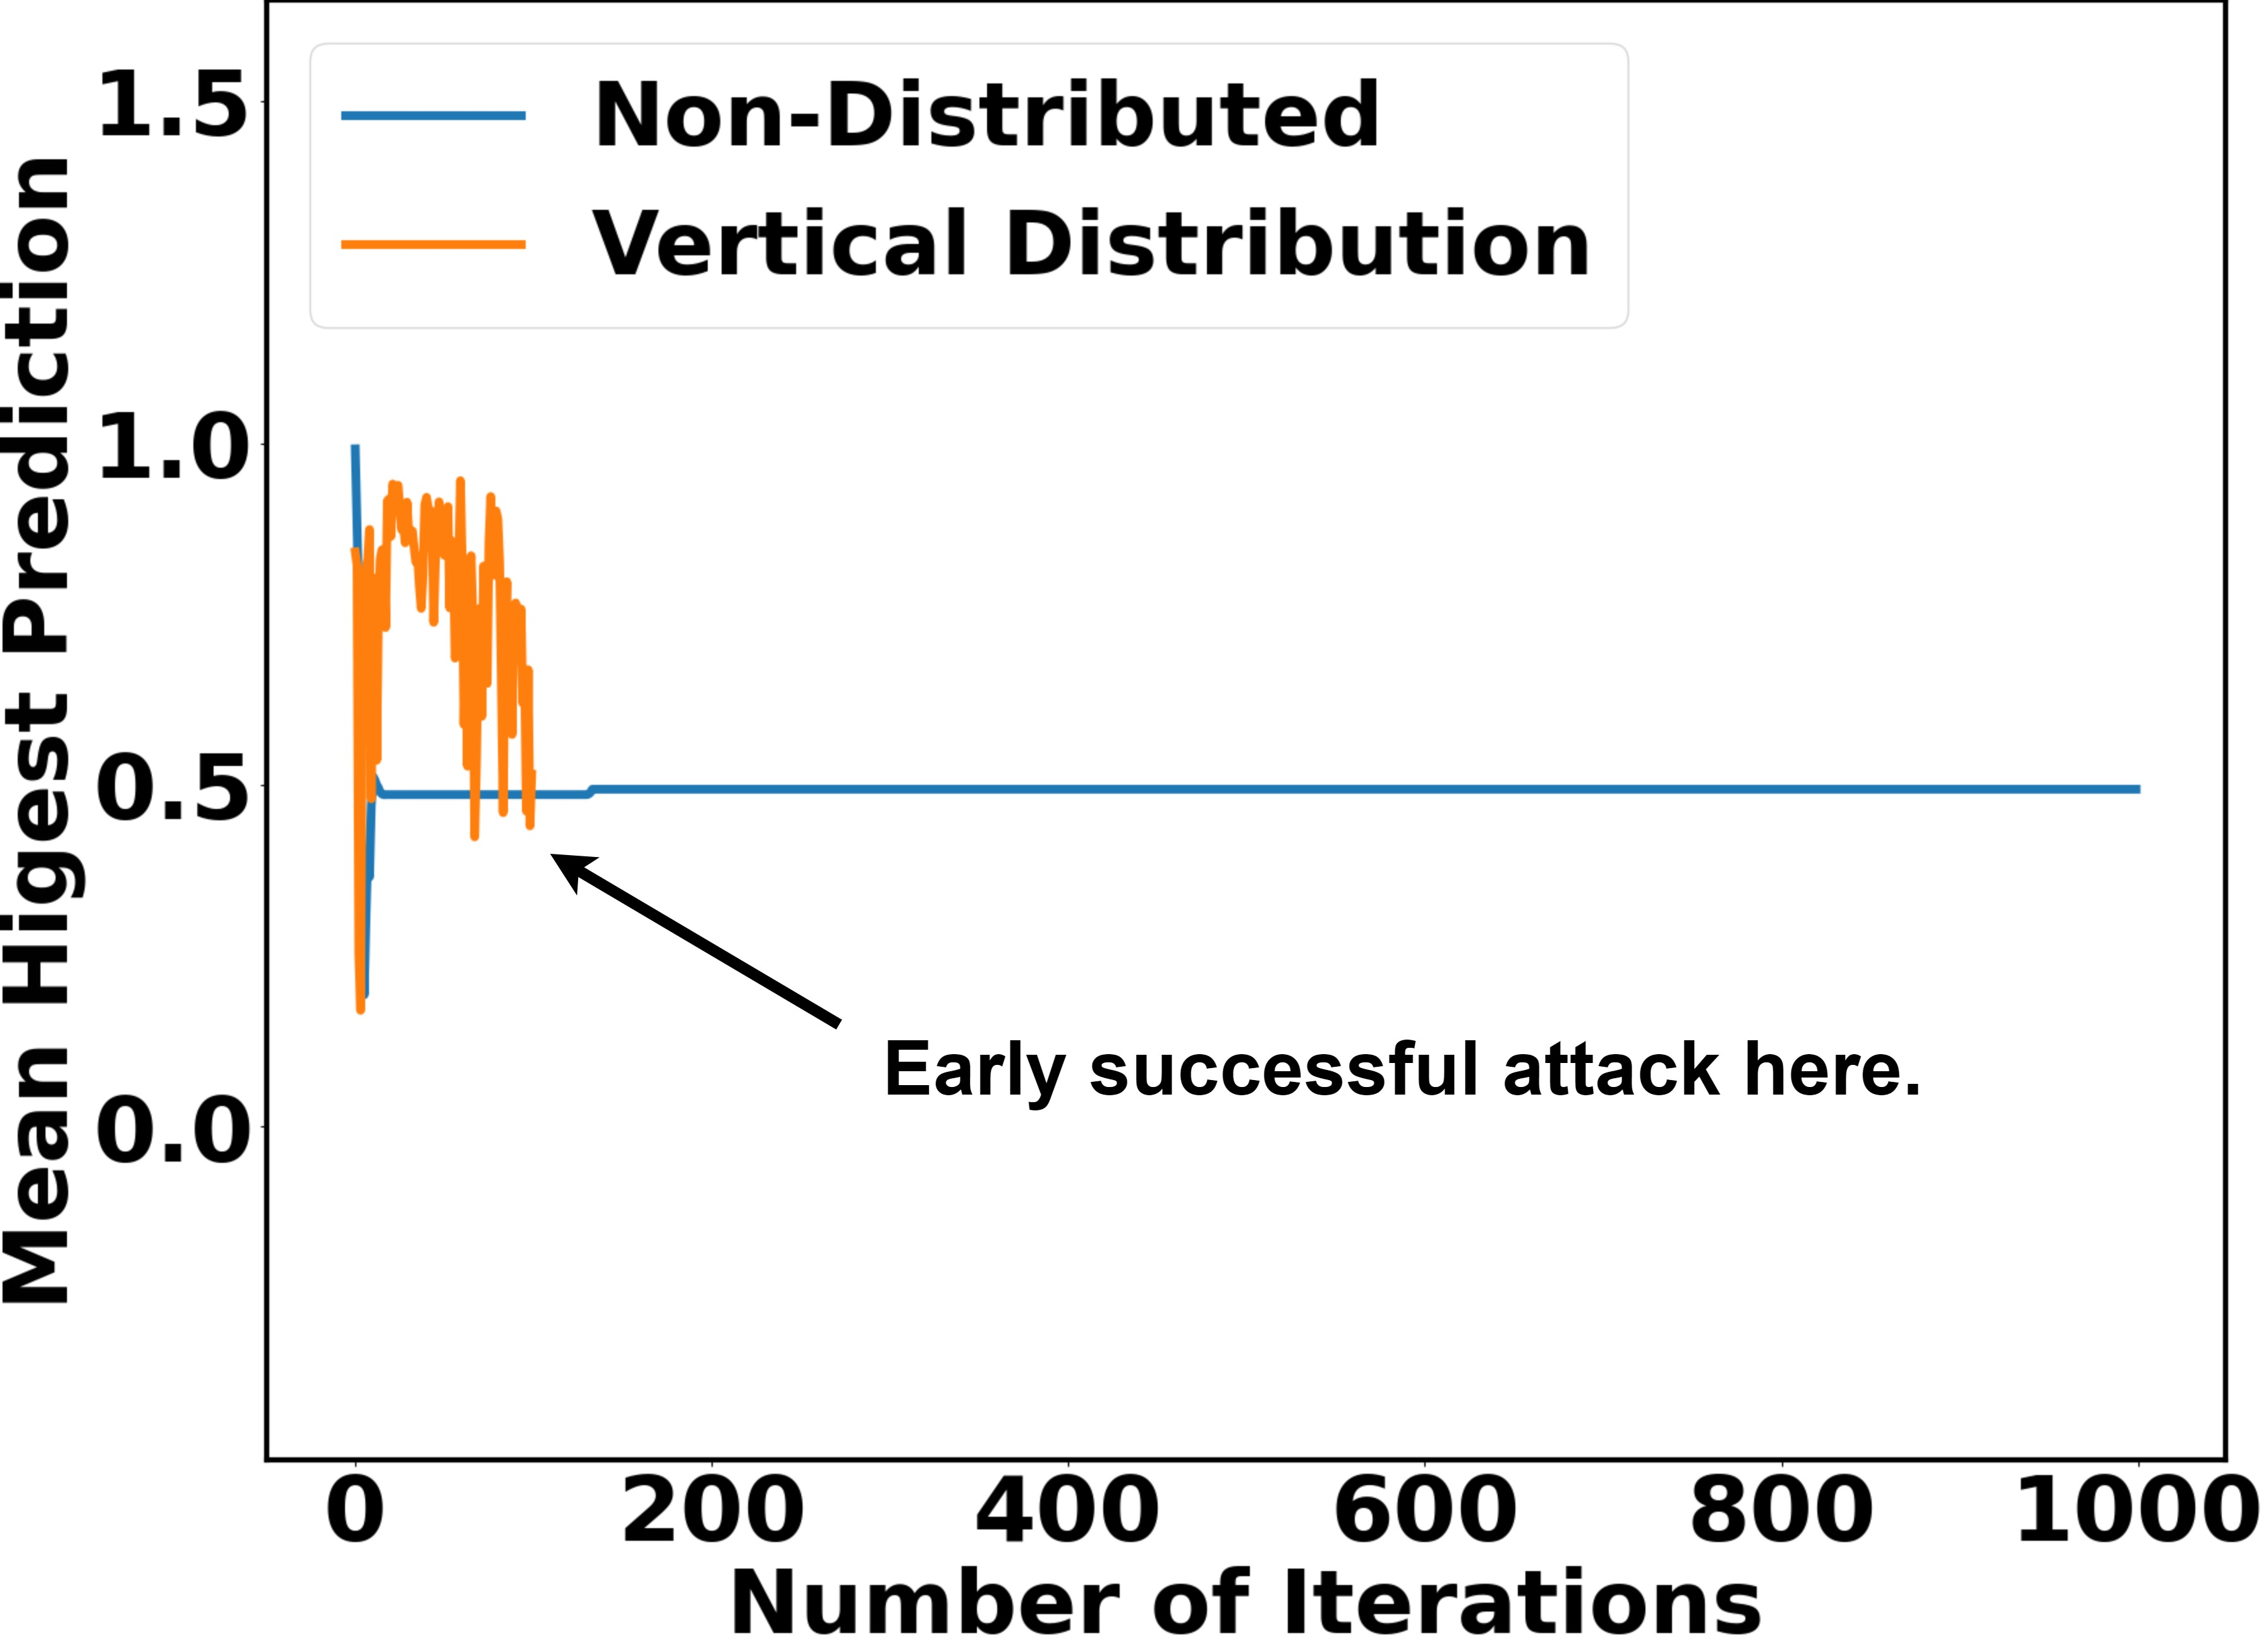
\includegraphics[width=\textwidth]{figures/chapter_classification/bandits_attack_vertical_margin.png}
    \caption{Bandits Attack (Gradient Estimation)}
    \label{fig:bandits_plot}
\end{subfigure}
\caption{The iteration process of different black-box attacks using vertical distribution.}
\label{fig.vertical_plot}
\end{figure*}


\begin{figure*}[tp]
\centering
\begin{subfigure}[t]{0.31\textwidth}
    \centering
    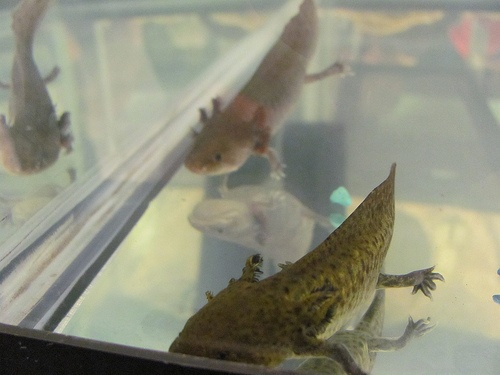
\includegraphics[width=\textwidth]{figures/chapter_classification/x_29_adv_simba_1.jpg}
    \caption{SimBA (No Distribution)}
    \label{fig:simba_no_img}
\end{subfigure}
\hfill
\begin{subfigure}[t]{0.31\textwidth}
    \centering
    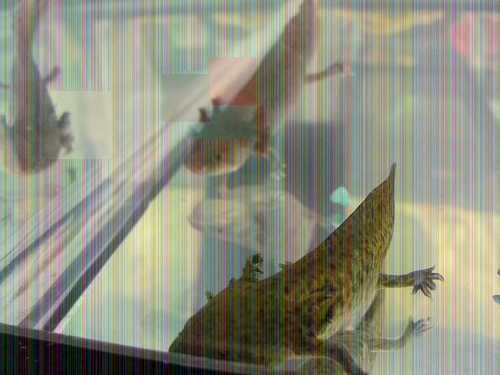
\includegraphics[width=\textwidth]{figures/chapter_classification/x_29_adv_square_1.jpg}
    \caption{Square Attack (No Distribution)}
    \label{fig:square_no_img}
\end{subfigure}
\hfill
\begin{subfigure}[t]{0.31\textwidth}
    \centering
    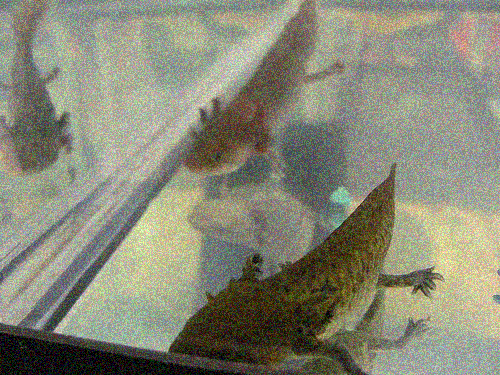
\includegraphics[width=\textwidth]{figures/chapter_classification/x_29_adv_bandits_1.jpg}
    \caption{Bandits Attack (No Distribution)}
    \label{fig:bandits_no_img}
\end{subfigure}
\hfill
\begin{subfigure}[t]{0.31\textwidth}
    \centering
    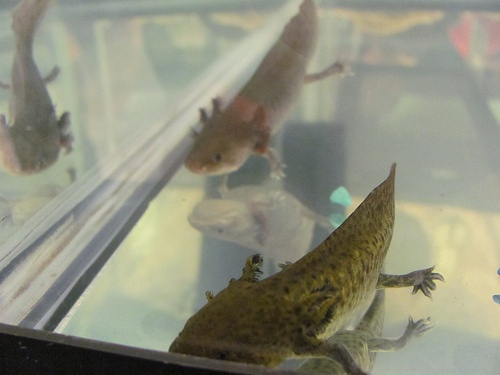
\includegraphics[width=\textwidth]{figures/chapter_classification/x_29_adv_simba_8.jpg}
    \caption{SimBA (Vertical)}
    \label{fig:simba_vertical_img}
\end{subfigure}
\hfill
\begin{subfigure}[t]{0.31\textwidth}
    \centering
    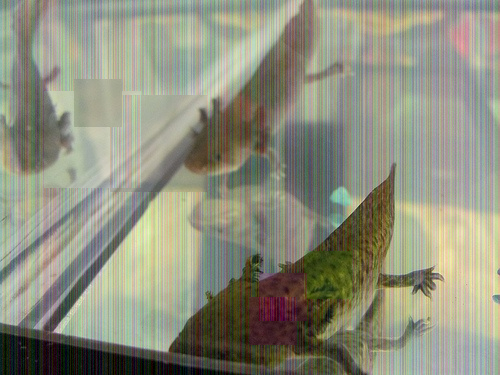
\includegraphics[width=\textwidth]{figures/chapter_classification/x_29_adv_square_8.jpg}
    \caption{Square Attack (Vertical)}
    \label{fig:square_vertical_img}
\end{subfigure}
\hfill
\begin{subfigure}[t]{0.31\textwidth}
    \centering
    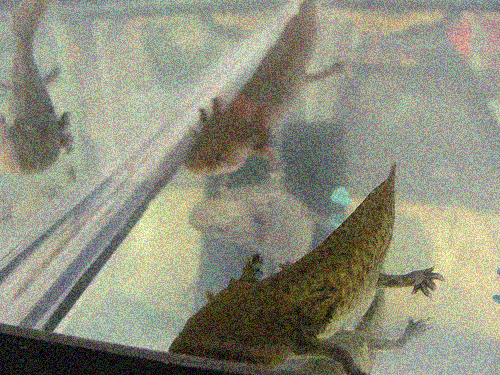
\includegraphics[width=\textwidth]{figures/chapter_classification/x_29_adv_bandits_8.jpg}
    \caption{Bandits Attack (Vertical)}
    \label{fig:bandits_vertical_img}
\end{subfigure}
\caption{Adversarial examples generated by different black-box attacks.}
\label{fig.vertical_img}
\end{figure*}

\section{Conclusion}

Our research presents a novel approach to accelerating black-box attacks against online cloud services by exploiting load balancing. We introduce two general frameworks, horizontal and vertical distribution, that can be applied to existing black-box attacks to reduce the total attack time significantly. To validate the efficiency of the frameworks, we conduct experiments using three black-box attacks against three commonly used image classification models.

Additionally, we contribute to the research community by open-sourcing our image classification cloud service, DeepAPI, to enable future research on distributed black-box attacks and provide insights into the practical threats posed by adversarial attacks against machine learning models deployed on cloud servers.

% \afterpage{\blankpage}

% \clearpage

% \section{The Black-box Adversarial Toolbox (BAT)}
% \label{sec:bat}

% We integrate distributed black-box attack methods into the Black-box Adversarial Toolbox (BAT). The objective is to achieve practical black-box attacks within limited queries and time.

% \begin{figure}[H]
% \centering
% 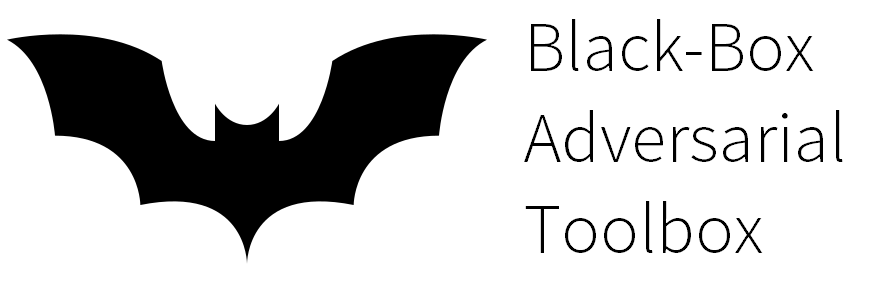
\includegraphics[scale=0.35]{figures/chapter_classification/bat.png}
% \caption{The Black-box Adversarial Toolbox}
% \label{fig.bat}
% \end{figure}

% Our demo application demonstrates that the original SimBA attack against a tiny VGG16 model pre-trained on the Cifar10 dataset takes around 200 seconds to achieve one successful attack. While the distributed SimBA attack takes only 40 seconds, which is five times faster. The acceleration ratio could grow even more as the number of nodes increases.

% \begin{figure}[H]
% \centering
% 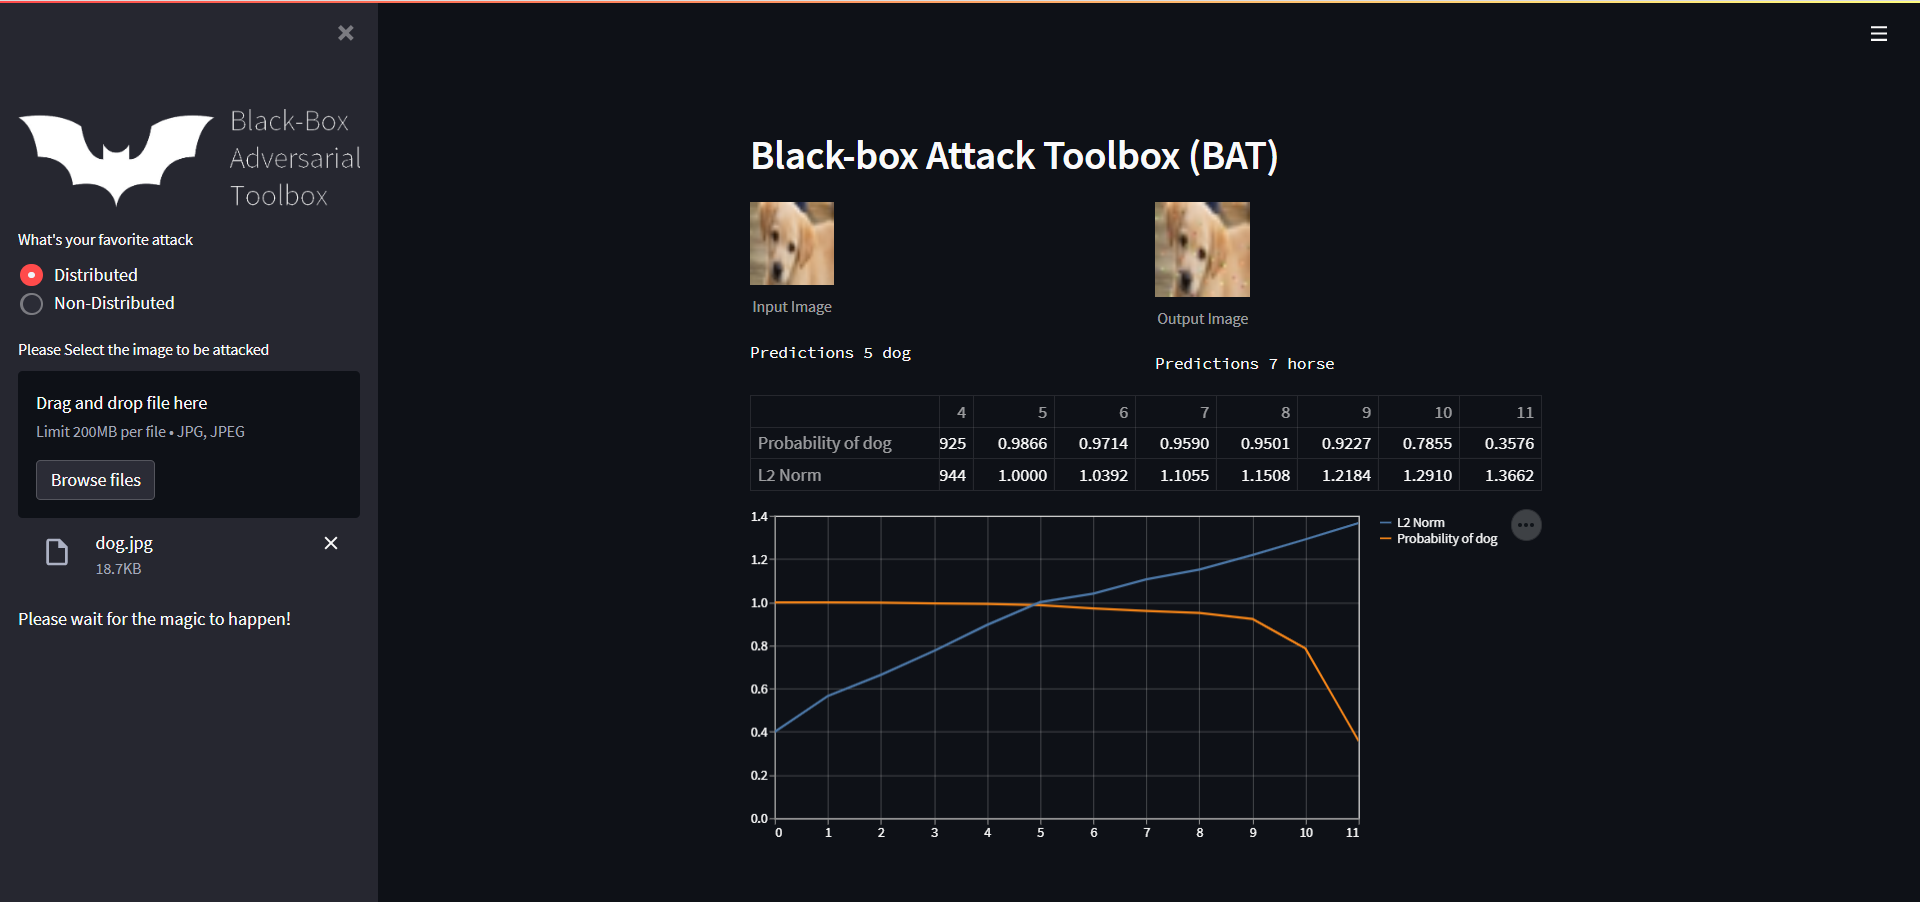
\includegraphics[width=0.75\textwidth]{figures/chapter_classification/bat_app.png}
% \caption{Demon application of the Black-box Adversarial Toolbox}
% \label{fig.bat_app}
% \end{figure}

% \clearpage

% \printbibliography[
%   keyword={chapter_classification}, heading=subbibintoc, resetnumbers=true
% ]